\documentclass{article}
\usepackage{nips14submit_e,times}

\title{Pure Exploration of Combinatorial Bandits}
\author{Shouyuan Chen}
\date{\today}
%%%%%%%%%%%%%%%%%%%%%%%%%%%%%%%%%%%%%%%%%%%%%%%%%%%%%%%%%%%%%

% Change "article" to "report" to get rid of page number on title page
\usepackage{amsmath,amsfonts,amsthm,amssymb}
\usepackage{setspace}
\usepackage{Tabbing}
\usepackage{fancyhdr}
\usepackage{lastpage} 
\usepackage{extramarks}
\usepackage{chngpage}
\usepackage{soul,color}
\usepackage{graphicx,float,wrapfig}
\usepackage{afterpage}
\usepackage{abstract}
\usepackage[colorlinks=true,linkcolor=blue,citecolor=blue]{hyperref}
\usepackage[numbers]{natbib}
\usepackage{algpseudocode}
\usepackage{algorithm}
\usepackage{xspace}
\usepackage{subcaption}
\usepackage{theoremref}
\usepackage{thmtools}
\usepackage{thm-restate}
\usepackage{cleveref}
%\usepackage{titling}


\allowdisplaybreaks

%%%%%%%%%%%%%%%%%%%%%%%%%%%%%%%%%%%%%%%%%%%%%%%%%%%%%%%%%%%%%
% Some tools
\newcommand{\junk}[1]{}

%\newtheorem{define}{Definition}
%\newtheorem{example}{Example}
%\newtheorem{lemma}{Lemma}
%\newtheorem{corollary}{Corollary}
%\newtheorem{theorem}{Theorem}

\declaretheorem{theorem}
\declaretheorem{lemma}
\declaretheorem{corollary}
\declaretheorem{define}
\declaretheorem{example}
\declaretheorem[name=Fact,Refname={Fact,Facts}]{fact}

%\def\ttdefault{blg}

\newcommand{\Algorithm}{{\small \textsf{CGapExp}}\xspace}
\newcommand{\AlgorithmPAC}{{\small \textsf{CGapExpPAC}}\xspace}
\newcommand{\Problem}{{\small \textsf{ExpCMAB}}\xspace}
\newcommand{\Rew}{\varphi}
\newcommand{\E}{\mathbb E}

\newcommand{\M}{\mathcal M}
\newcommand{\mmatch}{\mathcal M_{\mathsf{MATCH}}}
\newcommand{\mtop}{\mathcal M_{\mathsf{TOP}m}}
\newcommand{\mbandit}{\mathcal M_{\mathsf{BANDIT}m}}

\newcommand{\diff}{\mathsf{diff}}
\newcommand{\diffvalid}{\prec}
\newcommand{\B}{\mathcal B}
\newcommand{\C}{\mathcal C}
\newcommand{\del}{\backslash}

\newcommand{\RR}{\mathbb R}

%\newcommand{\vec}[1]{\mathbf #1}

\newcommand{\Bopt}{\mathcal B_{\mathsf{opt}}}
\newcommand{\Bmatch}{\mathcal B_{\mathsf{MATCH}}}
\newcommand{\Btop}{\mathcal B_{\mathsf{TOP}m}}
\newcommand{\Bbandit}{\mathcal B_{\mathsf{BANDIT}m}}

\DeclareMathOperator{\rank}{width}
\DeclareMathOperator{\rad}{rad}
\DeclareMathOperator{\decomp}{decomp}
\DeclareMathOperator*{\argmax}{arg\,max}
\DeclareMathOperator*{\argmin}{arg\,min}
\DeclareMathOperator{\Oracle}{Oracle}
\DeclareMathOperator{\Exchange}{Exchange}

\newcommand{\out}{\mathsf{Out}}


\let\Pr\undefined
\DeclareMathOperator{\Pr}{Pr}

\newcommand{\MultiIdent}{\textsc{Multi}\xspace}
\newcommand{\Matroid}{\textsc{Matroid}\xspace}
\newcommand{\Match}{\textsc{Match}\xspace}
\newcommand{\Path}{\textsc{Path}\xspace}

\newcommand{\inn}[1]{\left\langle #1 \right\rangle}
\newcommand{\nor}[1]{\left\|#1\right\|}
\renewcommand{\vec}[1]{\boldsymbol{#1}}

\renewcommand{\odot}{\circ}

%%%%%%%%%%%%%%%%%%%%%%%%%%%%%%%%%%%%%%%%%%%%%%%%%%%%%%%%%%%%%

\begin{document}
\newpage

\maketitle

\begin{abstract}
The abstract paragraph should be indented 1/2~inch (3~picas) on both left and
right-hand margins. Use 10~point type, with a vertical spacing of 11~points.
The word \textbf{Abstract} must be centered, bold, and in point size 12. Two
line spaces precede the abstract. The abstract must be limited to one
paragraph.
\end{abstract}

\section{Introduction}

The pure exploration problem is about designing strategies that make the best use of the limited budget.

\textbf{Motivation.}


\textbf{Contributions.}


Therefore, our results provide a complete characterization (within logarithmic factors) of the sample complexity for a large class of combinatorial problems, including \MultiIdent and \Matroid problem.
%In particular, we show that \Algorithm achieves an optimal sample complexity for these problems within logarithmic factors.

Our lower bound result also resolves the conjecture of \citet{kalyanakrishnan2012pac} on the lower bound sample complexity for the \MultiIdent problem.


%For a large class of combinatorial problems, including \MultiIdent and \Matroid problem, we give a complete characterization of 

\subsection{Related Work}

\textbf{Notations.} 

\section{Pure Exploration of Combinatorial Bandits}


%Let $\vec u \in \RR^{n}$ be a vector. 
% and $M\subseteq [n]$ be a set. 

\textbf{\Problem: problem formulation.}
Suppose that there are $n$ arms and the arms are numbered $1,2,\ldots,n$.
Each arm $e\in[n]$ is associated with a reward distribution $\Rew_e$ and define $w(e)=\E_{X\sim \Rew_e}[X]$ be the expected reward. 
Let $\vec w = \big(w(1),\ldots, w(n)\big)^T$ denote the vector of expected rewards.

Let $\M\subseteq 2^{[n]}$ be the family of all feasible solutions to a combinatorial problem.
%Let $M_* = \argmax_{M\in \M} w(M)$ denote the optimal set of arms which max
A learner wants to find the optimal solution of $\M$ which maximizes the expected reward $M_*=\argmax_{M\in \M} w(M)$ by playing the following game.
%The learning problem of pure exploration combinatorial bandit can be formalized as a game between a learner and a stochastic environment, where the learner's goal is to find the optimal solution to the combinatorial problem which maximizes the sum of expected reward $M_* = \argmax_{M\in \M} w(M)$.
At the beginning of the game, the reward distributions $\{\Rew_e\}_{e\in[n]}$ are unknown to the learner.
Then, the game is played for multiple rounds;
on each round $t$, the learner pulls an arm $p_t\in [n]$ and observes a reward sampled from the associated reward distribution $\Rew_{p_t}$.
The game continues until certain stopping condition is satisfied.
%which will be specified later.
After the game finishes, the learner need to output a solution $\out \in \M$.
%For the sake of simplicity, we shall assume that the optimal set $M_*$ is unique throughout the paper.

%Let $n$ denote the number of arms and suppose that the arms are numbered $1,2,\ldots,n$.

%We assume that all reward distributions are $R$-sub-Gaussian [].
%Notice that all distributions that are supported on $[0,R]$ are $R$-sub-Gaussian distributions [] and therefore our model subsumes the cases of bounded rewards.
%Let $w(e)=\E_{X\sim \Rew_e}[X]$ denote the expected reward of arm $e$ and let $\vec w = \big(w(1),\ldots,w(n)\big)^T$ denote the vector of expected rewards.
%In addition, for any set of arms $M\subseteq [n]$, we define $w(M) = \sum_{e\in M} w(e)$ as the sum of expected rewards of arms that belong to $M$.

%Notice that, if $\epsilon = 0$, then the learner is required to identify the optimal set, i.e. $\out = M_*$.



%\textbf{Fixed confidence and fixed budget.} 
We consider two different stopping conditions of the game, which are known as \emph{fixed confidence} setting and \emph{fixed budget} setting.
In the fixed confidence setting, the learner can stop the game at any point and her goal is to achieve a fixed confidence about the optimality of the returned set while uses a small number of pulls.
Specifically, given a confidence parameter $\delta$, the learner need to guarantee that $\Pr[\out = M_*] \ge 1-\delta$.
The performance is evaluated by the number of pulls used by the learner.
%Notice that the learner can stop the game at any point in this setting.
In the fixed budget setting, the game stops after a fixed number rounds.
The learner tries to minimize the probability of error $\Pr[\out \not= M_*]$ within these rounds.
In this case, the learner's performance is measured by the probability of error.


\textbf{Examples of combinatorial problems.} 
The formulation of the \Problem problem covers many online learning tasks.
We consider the following problems as examples.
\begin{itemize}
\item \MultiIdent.
\item \Matroid.
\item \Match.
\item \Path.
\end{itemize}

We assume that all reward distributions have $R$-sub-Gaussian tails. 
Formally, for all $t\in \RR$, we assume that $\mathbb E_{X\sim \Rew_e}\big[\exp(tX-tw(e))\big] \le \exp(R^2t^2/2)$.
It is well known that all distributions that are supported on $[0,R]$ satisfy this property [].
%Finally, for the sake of simplicity, we will assume that the optimal solution $M_*$ is unique.

%\textbf{Useful notations.}
%For any vector $\vec v\in \RR^n$ and any set $M \subseteq [n]$, we define $v(M) = \sum_{e\in M} v(e)$.


\section{Algorithm and Main Result}
%Our main contribution is an algorithm for solving the \Problem problem.
%Our algorithm 

%In this section, we describe our algorithm for pure exploration combinatorial bandit problem.
%Then, we analyze the sample complexity and the probability of error of our algorithm.

In this section, we present \Algorithm, a learning algorithm for the \Problem problem in the fixed confidence setting, and analyze its sample complexity. 
%Then, we analyze the sample complexity of \Algorithm algorithm.
The \Algorithm algorithm can be extended to the fixed budget and PAC learning settings. 
We will discuss these extensions in Section~\ref{section:extensions}.

%Many common combinatorial problems admit computationally efficient oracles.

\textbf{Oracle.}
We allow the \Algorithm algorithm to access a \emph{maximization oracle}. 
A maximization oracle takes a weight vector $\vec v \in \RR^{n}$ as input and computes an optimal solution with respect to the weight vector $\vec v$.
Formally, we call a function $\text{Oracle:}~\RR^{n} \rightarrow \M$ a maximization oracle if, for all $\vec v\in \RR^{n}$, we have $\Oracle(\vec v) \in \argmax_{M\in \M} v(M)$.
It is clear that a very broad class of combinatorial problems admit such maximization oracles.
Besides the access to the oracle, \Algorithm does not need \emph{any} additional knowledge of the combinatorial problem $\M$.

%For most non-trivial combinatorial problems, the size of the collection of feasible sets $\M$ is exponential in $n$.
%Hence, the definition of $\M$ 
%Therefore, the learning algorithm needs a succinct representation of $\M$.
%In particular, we allow the learning algorithm to use a \emph{maximization oracle} which can find the optimal set $M\in \M$ when the expected reward of each arm is known.
%Specifically, we assume that there exists an oracle which takes a vector $\vec v = \big(v(1),\ldots,v(n)\big)^T$ as input and returns a set $\Oracle(\vec v) = \argmax_{M\in \M} v(M)$.


\textbf{Algorithm.} 
%
%Our algorithm works for both fixed confidence and fixed budget settings.
%In either settings, the behaviors of our algorithm only differ in the construction of confidence radius and the stopping condition.
%In the following, we describe the procedure of our algorithm.
The \Algorithm algorithm maintains empirical mean $\bar w_t(e)$ and confidence radius $\rad_t(e)$ for each arm $e\in[n]$ and each round $t$.
The construction of confidence radius ensures that $|w(e)-\bar w_t(e)| \le \rad_t(e)$ holds with high probability for each arm $e \in [n]$ and each round $t>0$.
\Algorithm begins with an initialization phase in which each arm is pulled once.
Then, at round $t \ge n$, \Algorithm uses the following procedure to choose an arm to play. 
First, \Algorithm calls the oracle which computes the solution $M_t=\Oracle(\vec {\bar w}_t)$. 
The solution $M_t$ is the ``best'' solution with respect to the empirical means $\vec {\bar w}_t$.
% which maximizes empirical means $\bar w_t$ up to  $t$.
Then, \Algorithm explores possible refinements of $M_t$. 
In particular, \Algorithm uses the confidence radius to compute an adjusted expectation vector $\vec {\tilde w}_t$ in the following way: for each arm $e \in M_t$, $\tilde w_t(e)$ equals to the lower confidence bound $\tilde w_t(e) = \bar w_t(e)-\rad_t(e)$; and for each arm $e\not\in M_t$, $\tilde w_t(e)$ equals to the upper confidence bound $\tilde w_t(e)=\bar w_t(e)+\rad_t(e)$.
Intuitively, the adjusted expectation vector $\vec {\tilde w}_t$ penalizes arms belonging to the current solution $M_t$ and encourages exploring arms out of $M_t$.
\Algorithm then calls the oracle using the adjusted expectation vector $\vec {\tilde w}_t$ as input to compute a refined solution $\tilde M_t = \Oracle(\vec {\tilde w}_t)$.
If $\tilde w_t(\tilde M_t) = \tilde w_t(M_t)$ then \Algorithm stops and returns $\out=M_t$.
Otherwise, \Algorithm pulls the arm belonging to the symmetric difference $(\tilde M_t \del M_t) \cup (M_t \del \tilde M_t)$ between $M_t$ and $\tilde M_t$ with the largest confidence radius in the end of round $t$.
The pseudo-code of \Algorithm is shown in Algorithm~\ref{algo:pac}. 


\begin{algorithm}[htbp]
\begin{algorithmic}[1]
\Require Confidence parameter: $\delta \in (0,1)$; Maximization oracle: $\Oracle(\cdot): \RR^n \rightarrow \M$.
\Statex \textbf{Initialize:} Play each arm $e \in [n]$ once. Initialize empirical means $\vec {\bar w}_n$ and set $T_{n}(e) \gets 1$ for all $e$.
\For{$t=n,n+1,\ldots$}
	\State $M_t \gets \Oracle(\vec {\bar w}_t)$
	\For{$e\in [n]$}
		\If {$e\in M_t$}
			\State $\tilde w_t(e) \gets \bar w_t(e)-\rad_t(e)$
		\Else
			\State $\tilde w_t(e) \gets \bar w_t(e)+\rad_t(e)$
		\EndIf
	\EndFor
	\State $\tilde M_t \gets \Oracle(\vec{\tilde w}_t)$
	\If{$\tilde w_t(\tilde M_t) = \tilde w_t(M_t)$}
		\State $\out \gets M_t$
		\State \textbf{return} $\out$
	\EndIf
	\State $p_t \gets \argmax_{e\in (\tilde M_t \del M_t) \cup (M_t \del \tilde M_t)} \rad_t(e)$\label{algo:step:D}
	\State Pull arm $p_t$ and observe the reward
	\State Update empirical means $\vec {\bar w}_{t+1}$ using the observed reward
	\State Update number of pulls: $T_{t+1}(p_t)\gets T_{t}(p_t)+1$ and $T_{t+1}(e) \gets T_{t}(e)$ for all $e\not=p_t$
	\EndFor
\end{algorithmic}
\caption{\Algorithm: Combinatorial Gap Exploration}
\label{algo:pac}
\end{algorithm}


\subsection{Analysis}
%In this part, we analyze the performance of Algorithm~\ref{algo:pac} for both fixed confidence and fixed budget settings. 
Now we prove a problem-dependent sample complexity bound of the \Algorithm algorithm. 
Our sample complexity bound depends on several combinatorial properties of $\M$. 
Therefore, to state our result, we first introduce notions to capture these properties.
%To state our results, we need to define two quantities: gap and width.

\textbf{Gap.} We begin with defining a hardness complexity measure of the \Problem problem. 
For each arm $e \in [n]$, we define gap $\Delta_e$ as
\begin{equation}
\label{eq:define-delta}
\Delta_e = \begin{cases}
			   w(M_*)-\max_{M\in \M: e\in M} w(M) & \text{if } e\not \in M_*, \\
			   w(M_*)-\max_{M\in \M: e\not \in M} w(M) & \text{if } e\in M_*,
			\end{cases}
\end{equation}
where we use the convention that the maximum value of an empty set is $-\infty$. 
%Therefore the gap $\Delta_e$ of a redundant arm $e\not \in M$ for all $M\in \M$ is $+\infty$.
We also define the hardness $\mathbf H$ as the sum of inverse squared gaps 
\begin{equation}
\label{eq:hardness}
\mathbf H =\sum_{e\in [n]} \Delta_e^{-2}.
\end{equation}

From Eq.~\eqref{eq:define-delta}, we see that, for each arm $e\not\in M_*$, $\Delta_e$ represents the gap between the optimal set $M_*$ and the best set that includes arm $e$; and, for each arm $e\in M_*$, $\Delta_e$ is the sub-optimality of the best set that does not include arm $e$.
%We notice that, for many combinatorial problems, the definition Eq.~\eqref{eq:define-delta} naturally reflects the hardness of an arm.
%().
%Figure X illustrates these interpretations.
We notice that this definition resembles the previous definition of gaps for the \MultiIdent problem \citep{kalyanakrishnan2012pac,gabillon2012best}.



\textbf{Exchange class and the width of $\M$.} 
The analysis of our algorithm depends on certain exchange properties of combinatorial structures.
To capture these properties, we introduce notions of \emph{exchange set} and \emph{exchange class} as tools for our analysis.
We present their definitions in the following.

%An exchange set is defined as a pair of disjoint sets.

We begin with the definition of exchange set. 
We define an exchange set $b$ as an ordered pair of disjoint sets $b=(b_+,b_-)$ where $b_+\cap b_- = \emptyset$.
Then, we define operator $\oplus$ such that, for any set $M$ and any exchange set $b=(b_+,b_-)$, we have $M\oplus b \triangleq M\del b_- \cup b_+$.
Similarly, we also define operator $\ominus$ such that $M\ominus b \triangleq M\del b_+\cup b_-$.

We call a family of exchange sets $\B$ an \emph{exchange class for $\M$} if $\B$ satisfies the following property.
Let $M$ and $M'$ be two  elements of $\M$.
Then, for any $e \in (M\del M')$, there exists an exchange set $(b_+,b_-)\in \B$ which satisfies $e\in b_-$, $b_+ \subseteq M'\del M$, $b_- \subseteq M \del M'$, $(M\oplus b) \in \M$ and $(M'\ominus b) \in \M$.
We define the \emph{width} of exchange class $\B$ to be the size of largest exchange set as follows
\begin{equation}
\label{eq:width}
\rank(\B) = \max_{(b_+,b_-) \in \B} |b_+|+|b_-|.
\end{equation}

%An exchange class can be seen as a set operations that transform one feasible set to another.
Intuitively, for any feasible sets $M$ and $M'$, there exists an exchange set $(b_+,b_-)\in \B$ belonging to the exchange class $\B$ which can be seen as an ``operation'' that transforms $M$ one step towards $M'$: this operation generates a new feasible set $M\oplus b$ by removing elements (including $e$) from $M$ and adding elements which belongs to $M'$.
%Therefore, for any two elements $M,M'$ of $\M$, one can sequentially apply a finite number of these operations of $\B$ to transform $M$ to $M'$.it
One can chain these operations together: for any $M\not= M'$, there exists a sequence of exchange sets $b_1,\ldots, b_k$ of $\B$ such that $M'=M\oplus b_1 \oplus \ldots \oplus b_k$.

We notice that an exchange class for $\M$ can be ``redundant''. 
It may contains some unnecessary exchange set $b$, such that $M\oplus b \not\in \M$ for any $M \in \M$.
These redundant exchange sets do not affect our analysis.
But allowing them would simplify the construction and description of exchange classes for certain combinatorial problems.
%On the other hand, this also means that, for a fixed combinatorial problem, there exist many exchange classes.
%In particular, we are interested with the exchange classes with small widths.


%For a fixed combinatorial problem $\M$, the exchange classes for $\M$ are not unique.
Finally, let $\Exchange(\M)$ denote the collection of all possible exchange classes for $\M$.
%We are interested with the exchange class with small width.
We define the width of a combinatorial problem $\M$ as the width of the thinnest exchange class
$$
\rank(\M) = \min_{\B \in \Exchange(\M)} \rank(\B).
$$


\junk{
Next, we investigate the exchange classes for our running examples.
For \MultiIdent problem, we can construct the exchange class as $\B_{1}=\{(\{i\},\{j\})\;|\;\forall i\in [n], j\in [n]\}$.
It is easy to verify $\B_{1}$ is an exchange class for $\M_{\MultiIdent}$: one can transform a set of $k$ elements to another by adding and removing an element for each time.
In fact, a standard result from matroid theory, called basis exchange property (see Lemma~\ref{lemma:basis-exchange-matroid} in the appendix), shows that $\B_1$ is also an exchange class for the more general \Matroid problem.
%From Lemma~\ref{lemma:basis-exchange-matroid}, we see that $\B_1$ is an exchange class for $\M_{\Matroid}$.
Next, for \Match problem, an exchange class contains all cycles of the graph $G$.
Given two matchings $M,M'$, the union $M\cup M'$ is a union of disjoint cycles [].
These cycles are known to be augmenting cycles in combinatorial optimization literature [].
Figure~Y illustrates these exchanges classes.
}

For many problems, the exchange classes with small widths corresponding to natural combinatorial structures. 
To see this, we construct the exchange classes for our running examples.
Our constructions are summarized in \Cref{lemma:example-exchange-class}.
\begin{fact}
There exist exchange classes $\B_{\MultiIdent}$, $\B_{\Matroid}$, $\B_{\Match}$ and $\B_{\Path}$ for $\M_{\MultiIdent}$, $\M_{\Matroid}$, $\M_{\Match}$ and $\M_{\Path}$, respectively. 
These exchange classes can be constructed as follows
\begin{enumerate}
	\item $\B_{\MultiIdent}=\big\{(\{i\},\{j\})\;|\;\forall i\in [n], j\in [n]\big\}$.
	\item $\B_{\Matroid}=\big\{(\{i\},\{j\})\;|\;\forall i\in [n], j\in [n]\big\}$.
	\item $\B_{\Match}=\big\{(C_+,C_-)\;|\; C_+\cup C_- \text{ is a cycle of }G\big\}$.
	\item $\B_{\Path}=\big\{ (P_1, P_2) \;|\;P_1,P_2\text{ are two disjoint paths of }G\text{ with same endpoints}\big\}$.
\end{enumerate}
In addition, we have $\rank(\B_{\MultiIdent})=2$, $\rank(\B_{\Matroid})=2$, $\rank(\B_{\Match})=|V|$ and $\rank(\B_{\Path})=|V|$.
This means that $\rank(\M_\MultiIdent)\le 2$, $\rank(\M_\Matroid) \le 2$, $\rank(\M_\Match) \le |V|$ and $\rank(\M_\Path) \le |V|$.
\label{lemma:example-exchange-class}
\end{fact}
We illustrate these  exchanges classes in \Cref{fig:exchange}.
The construction for \MultiIdent problem is straightforward.
For \Matroid problem, we leverage the basis exchange property of matroids (see Lemma~\ref{lemma:basis-exchange-matroid} in the supplementary material).
And for \Match and \Path problems, we use standard graph-theoretical properties of matchings and paths.
A detailed proof of \Cref{lemma:example-exchange-class} is deferred to the supplementary material.

\begin{figure}
\centering
\begin{subfigure}[c]{0.22\textwidth}
	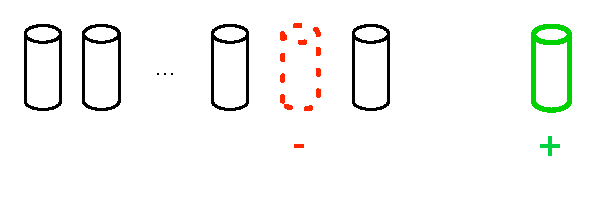
\includegraphics[width=\textwidth]{fig/exchange-multi}
	\caption{An element of $\B_{\MultiIdent}$.}
\end{subfigure}
~
\begin{subfigure}[c]{0.25\textwidth}
	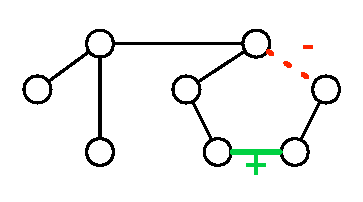
\includegraphics[width=\textwidth]{fig/exchange-matroid}
	\caption{An element of $\B_{\Matroid}$}
	\label{fig:exchange:matroid}
\end{subfigure}
~
\begin{subfigure}[c]{0.22\textwidth}
	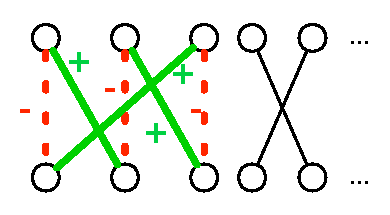
\includegraphics[width=\textwidth]{fig/exchange-match}
	\caption{An element of $\B_{\Match}$.}
\end{subfigure}
~
\begin{subfigure}[c]{0.22\textwidth}
	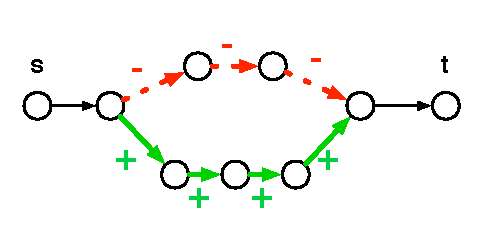
\includegraphics[width=\textwidth]{fig/exchange-path}
	\caption{An element of $\B_{\Path}$.}
\end{subfigure}
\caption{
Examples of exchange sets belonging to the exchange classes $\B_{\MultiIdent}$, $\B_{\Matroid}$, $\B_{\Match}$ and $\B_{\Path}$:
green-solid elements constitute the set $b_+$, red-dotted elements constitute the set $b_-$ and the example exchange set is $b=(b_+,b_-)$. 
(In \Cref{fig:exchange:matroid}, we consider spanning tree as a specific instance for the \Matroid problem.)
}
\label{fig:exchange}
\end{figure}

\textbf{Main result.} 
Our main result is a problem-dependent sample complexity bound of the \Algorithm algorithm.
In particular, we show that \Algorithm returns the optimal set with high probability and uses at most $\tilde O\big(\rank(\M)^2 \mathbf H\big)$ samples.
\begin{restatable}{theorem}{mainresult}
Given any $\delta \in (0,1)$, any $\M \subseteq 2^{[n]}$ and any $\vec w \in \RR^{n}$.
Assume that the reward distribution $\Rew_e$ for each arm $e\in [n]$ is  $R$-sub-Gaussian with mean $w(e)$.
%Let $\B$ be an exchange class for $\M$ and let $\{\Delta_e\}_{e\in [n]}$ be the gaps defined in Eq.~\eqref{eq:define-delta}.
Set $\rad_t(e) = R\sqrt{\frac{2\log\left(\frac{4n t^2}\delta\right)}{T_e(t)}}$ for all $t > 0$ and $e\in[n]$.
Then, with probability at least $1-\delta$, the \Algorithm algorithm (Algorithm~\ref{algo:pac}) returns the optimal set $\out=M_*$ and
\begin{equation}
\label{eq:sample-complexity}
T \le O\left(R^2\rank(\M)^2\mathbf H\log\left(R^2\rank(\M)^2\mathbf H \cdot n/\delta\right)\right),
\end{equation}
where $T$ denotes the number of samples used by Algorithm~\ref{algo:pac} and $\mathbf H$ is defined in Eq.~\eqref{eq:hardness}.
\label{theorem:main}
\end{restatable}
\junk{
By combining Lemma~\ref{lemma:example-exchange-class} and Theorem~\ref{theorem:main}, we can bound the sample complexity of \Algorithm for our running examples.
\begin{corollary}
\begin{itemize}
	\item \MultiIdent. $T \le O\big(\mathbf H \log(n\mathbf H/\delta)\big)$.
	\item \Matroid. $T \le O\big(\mathbf H \log(n\mathbf H/\delta)\big)$.
	\item \Match. $T \le O\big(|V|^2 \mathbf H \log(n |V|^2 \mathbf H/\delta)\big)$.
	\item \Path. $T \le O\big(|V|^2 \mathbf H \log(n |V|^2 \mathbf H/\delta)\big)$.
\end{itemize}
\end{corollary}
}

\textbf{Remarks.}
%Theorem~\ref{theorem:main} upper bounds the sample complexity of \Algorithm for an arbitrary combinatorial problem $\M$.
%We see that the sample complexity Eq.~\eqref{eq:sample-complexity} depends on $\rank(\B)$ and $\B$ is an arbitrary exchange class for $\M$.
%Therefore, the sample complexity Eq.~\eqref{eq:sample-complexity} is minimizes $\B$ 
%Notice that $\B$ does not 
%Theorem~\ref{theorem:main} is a general result which provides a sample complexity for any combinatorial problem $\M$.
For the \MultiIdent problem, we see that \Cref{lemma:example-exchange-class} shows that $\rank(\MultiIdent)=O(1)$.
Therefore, the sample complexity bound of \Algorithm is $O\big(\mathbf H \log(n\mathbf H/\delta)\big)$ for this problem.
This matches the previous problem-dependent bounds for the \MultiIdent problem \citep{kalyanakrishnan2012pac,gabillon2012best}.
%And Theorem~\ref{algo:pac} establishes the first sample complexity bound for the pure exploration of other combinatorial bandits.
For the \Matroid problem, we know that $\rank(\Matroid)=O(1)$ and hence the sample complexity is also $O\big(\mathbf H \log(n\mathbf H/\delta)\big)$.
For \Match and \Path problem, we see that the sample complexity is bounded by $\tilde O(|V|^2 \mathbf H)$.



%Many combinatorial problem $\M$ is associated with an exchange class with small width.


%From the definition, it is easy to see that if $\B$ is an exchange class, then, for any $M\not= M'$, there exists a sequence of exchange sets $b_1,\ldots, b_k$ belonging to $\B$ such that $M'=M\oplus b_1 \ldots \oplus b_k$.
%Hence, intuitively, an exchange class for $\M$ characterizes the ``operations'' of transforming an element $M\in \M$ to another element $M'\in \M$.



\section{Lower Bound}
In this section, we present a problem-dependent lower bound on the sample complexity of the \Problem problem. 
To state our results, we first define the notion of \emph{$\delta$-correct algorithm} as follows.
For any $\delta \in (0,1)$, we call an algorithm $\mathbb A$ a $\delta$-correct algorithm if, for any expected reward $\vec w \in \RR^{n}$, the probability of error of $\mathbb A$ is at most $\delta$, i.e. $\Pr[M_*\not =\out] \le \delta$, where $\out$ is the output of algorithm $\mathbb A$.

We show that, for any family of feasible solutions $\M$ and any expected rewards $\vec w$, any $\delta$-correct algorithm $\mathbb A$ must use at least $\Omega\big(\mathbf H \log(1/\delta) \big)$ samples in expectation.
\begin{restatable}{theorem}{lowerbound}
Fix any $\M\subseteq 2^{[n]}$ and any vector $\vec w \in \RR^n$.
Suppose that, for each arm $e\in [n]$, the reward distribution $\Rew_e$ is given by $\Rew_e=\mathcal N(w(e),1)$, where $\mathcal N(\mu, \sigma^2)$ denotes a Gaussian distribution with mean $\mu$ and variance $\sigma^2$. 
Then, for any $\delta \in (0,e^{-16}/4)$ and any $\delta$-correct algorithm $\mathbb A$, we have
\begin{equation}
\label{eq:lower-bound}
\E[T] \ge \frac{1}{16} \mathbf H \log\left(\frac{1}{4\delta}\right),
\end{equation}
where 
$T$ denote the number of total samples used by algorithm $\mathbb A$ and
$\mathbf H$ is defined in Eq.~\eqref{eq:hardness}.
\label{theorem:lower-bound}
\end{restatable}

%Now we compare the sample complexity Eq.~\eqref{eq:sample-complexity} of \Algorithm to the lower bound provided in Theorem~\ref{theorem:lower-bound} on our running examples \MultiIdent, \Matroid, \Match and \Path.
%For clarity, we consider the case that $\epsilon=0$ which corresponds to the learning problem of finding the optimal set.
%We see that \Algorithm algorithm uses at most $\tilde O(\rank(\B)^2 \mathbf H)$ samples.
%Recall that, for \MultiIdent and \Matroid, Lemma~\ref{lemma:example-exchange-class} shows that $\rank(\B)=2$.
Theorem~\ref{theorem:lower-bound} resolves  the conjecture of \citet{kalyanakrishnan2012pac} that the lower bound of sample complexity of \MultiIdent problem is $\Omega\big(\mathbf H\log(1/\delta)\big)$.
In addition, our upper bound Theorem~\ref{theorem:main} shows that, for \MultiIdent and \Matroid, the sample complexity of \Algorithm is $O(\mathbf H\log(n\mathbf H/\delta))$.
Hence,  we see that the \Algorithm algorithm achieves the optimal sample complexity within logarithmic factors for these two problems.

%On the other hand, for $\Match(V,E)$ and $\Path(V,E)$, we see that the gap between the upper bound Eq.~\eqref{eq:sample-complexity} and this lower bound is a factor of $|V|^2$.
On the other hand, for general combinatorial problems with non-constant widths, we see that there is a gap of $\tilde \Theta(\rank(\M)^2)$ between the upper bound Eq.~\eqref{eq:sample-complexity} and the lower bound Eq.~\eqref{eq:lower-bound}.
Ignoring the logarithmic factors, this gap only depends on the underlying combinatorial structure of $\M$.
This suggests that the sample complexity of \Algorithm has an optimal dependency on the hardness $\mathbf H$ up to logarithmic factors for general combinatorial problems.
Furthermore, we conjecture that the sample complexity lower bound might intrinsically depend on the size of exchange sets which is bounded by $\rank(\M)$. 
We provide evidence on this conjecture which lower bounds the sample complexity of exploration on exchange sets in the supplementary material.
 %dependency on $\rank(\M)$ of the sample complexity might be intrinsic. 
%In the supplementary material, we provide evidence showing that the sample complexity of any $\delta$-correct algorithm should be related to size of exchange sets. 


\section{Extensions}
\label{section:extensions}

\Algorithm is a general and flexible learning algorithm for the \Problem problem.
In this section, we present two extensions to \Algorithm that allow it to work in the fixed budget setting and PAC learning setting.

\subsection{Fixed Budget Setting}
\label{section:fixed-budget}
We can extend the \Algorithm algorithm to the fixed budget setting using two simple modifications: (1) requiring \Algorithm to terminate after $T$ rounds; and (2) using a different construction of confidence intervals.
The first modification ensures that \Algorithm uses at most $T$ samples, which meets the requirement of the fixed budget setting.
And the second modification bounds the probability that the confidence intervals are valid for all arms in $T$ rounds.
The following theorem shows that the probability of error of the modified \Algorithm is bounded by 
$O\left(Tn\exp\left(\frac{-T}{\rank(\M)^2\mathbf H} \right)\right)$.
\begin{restatable}{theorem}{resultbudget}
%Given any $T>0$, any combinatorial problem $\M \subseteq 2^{[n]}$ and any vector $\vec w \in \RR^{n}$.
%Assume that the reward distribution $\Rew_e$ for each arm $e\in [n]$ is  $R$-sub-Gaussian with mean $w(e)$.
%Let $\B$ be an exchange class for $\M$ and let $\{\Delta_e\}_{e\in [n]}$ be the gaps defined in Eq.~\eqref{eq:define-delta}.
Use the same notations as in Theorem~\ref{theorem:main}.
Given $T > n$ and parameter $\alpha > 0$, set the confidence radius $\rad_t(e) = R\sqrt{\frac{\alpha}{T_e(t)}}$ for all arms $e\in[n]$ and all $t>0$.
Run \Algorithm algorithm for at most $T$ rounds.
Then, for $0 \le \alpha \le \frac19 (T-n)\left(R^2\rank(\M)^2 \mathbf H\right)^{-1}$, we have
%the probability of error of \Algorithm is bounded as follows
\begin{equation}
\label{eq:fix-budget}
\Pr\big[\out\not=M_*\big] \le 2Tn\exp\left(-2\alpha\right).
\end{equation}
%In particular, when $\alpha=\frac19 (T-n)\left(R^2\rank(\M)^2 \mathbf H\right)^{-1}$, the probability of error is at most $O\Big(Tn\exp\left(-\frac{T}{\rank(\M)^2 \mathbf H}\right)\Big)$.
\label{theorem:main-budget}
\end{restatable}
The right-hand side of Eq.~\eqref{eq:fix-budget} equals to $O\left(Tn\exp\left(\frac{-T}{\rank(\M)^2\mathbf H} \right)\right)$
when parameter $\alpha = O(T\mathbf H^{-1}\rank(\M)^{-2})$.
For \MultiIdent problem, we see that this matches the guarantees of the previous fixed budget algorithm due to \citet{gabillon2012best}.

\subsection{PAC Learning}
Now we consider a setting where the learner is only required to report an approximately optimal set of arms. 
More specifically, we consider the notion of $(\epsilon,\delta)$-PAC algorithm.
Formally, an algorithm $\mathbb A$ is called an $(\epsilon,\delta)$-PAC algorithm if its output $\out$ satisfies $\Pr\big[w(M_*)-w(\out) > \epsilon\big] \le \delta$.

We show that a simple modification on the \Algorithm algorithm gives an $(\epsilon,\delta)$-PAC algorithm, with guarantees similar  to Theorem~\ref{theorem:main}.
In fact, the only modification needed is to change the stopping condition from $\tilde w_t(\tilde M_t)\le \tilde w_t(M_t)$ to $w(\tilde M_t)-w(M_t) \le \epsilon$ on line~\ref{algo:step:D} of Algorithm~\ref{algo:pac}.
We let  \AlgorithmPAC denote the modified algorithm.
In the following theorem, we show that \AlgorithmPAC is indeed an $(\epsilon,\delta)$-PAC algorithm and has sample complexity similar to \Algorithm.
\begin{restatable}{theorem}{resultpac}
Use the same notations as in Theorem~\ref{theorem:main}.
Fix $\delta\in(0,1)$ and $\epsilon \ge 0$.
Then, with probability at least $1-\delta$, the output $\out$ of \AlgorithmPAC satisfies
$
w(M_*)-w(\out) \le \epsilon.
$
In addition, the number of samples $T$ used by the algorithm satisfies
\begin{equation}
T \le 
O\left(R^2\sum_{e\in [n]} \min\left\{\frac{\rank(\M)^2}{\Delta_e^2}, \frac{K^2}{\epsilon^2}\right\} 
\log\left(\frac{R^2n}\delta \sum_{e\in [n]} \min\left\{\frac{\rank(\M)^2}{\Delta_e^2}, \frac{K^2}{\epsilon^2}\right\}\right)\right),
\label{eq:pac}
\end{equation}
where $K=\max_{M\in \M} |M|$ is the size of the largest feasible solution.
\label{theorem:pac}
\end{restatable}
We see that the sample complexity of \AlgorithmPAC decreases when $\epsilon$ increases.
And if $\epsilon=0$, the sample complexity Eq.~\eqref{eq:pac} of \AlgorithmPAC equals to that of \Algorithm. 

There are several PAC algorithms for the \MultiIdent problem in the literature with different guarantees \citep{kalyanakrishnan2012pac,zhou2014optimal,gabillon2012best}.
\citet{zhou2014optimal} proposed an $(\epsilon,\delta)$-PAC algorithm for the \MultiIdent problem with a problem-independent sample complexity bound of $O(\frac{K^2n}{\epsilon^2}+\frac{Kn\log(1/\delta)}{\epsilon^2})$.\footnote{We notice that \citet{zhou2014optimal} allow an $(\epsilon',\delta)$-PAC algorithm to produce an output with \emph{average} sub-optimality of $\epsilon'$. This is equivalent to our definition of $(\epsilon,\delta)$-PAC algorithm with $\epsilon=K\epsilon'$.}
% which is $\tilde O(\frac{K^2n}{\epsilon^2})$ after ignoring logarithmic factors.
If we ignore logarithmic factors, then the sample complexity bound of \AlgorithmPAC for the \MultiIdent problem is better than theirs $\tilde O(\sum_{e\in[n]}\min\{\Delta_e^{-2}, K^2\epsilon^{-2}\}) \le  \tilde O(nK^2\epsilon^{-2})$.
%Our bound is always smaller than or equal to the sample complexity bound $\tilde O(nK^2\epsilon^{-2})$ of \citet{zhou2014optimal}, regardless the value of gaps $\Delta_1,\ldots,\Delta_n$ and $\epsilon$.
On the other hand, the algorithms of \citet{kalyanakrishnan2012pac} and \citet{gabillon2012best} guarantee to find $K$ arms such that each of them is better than the $K$-th optimal arm within a factor of $\epsilon$ with probability $1-\delta$.
Unless $\epsilon=0$, their guarantee is different from ours which concerns the optimality of the sum of $K$ arms.
%though the bounds are similar, our definition of $(\epsilon,\delta)$-PAC algorithm is different from that of \citet{kalyanakrishnan2012pac,gabillon2012best}, where these work aim to 
 %$(\epsilon, \delta)$

%Our definitions of 
%For the \MultiIdent problem, 


%Notice that our sample complexity bound of PAC learning is not comparable to that of XXX. 
%Since their objective is to find $K$

\newpage
\bibliography{bandit}
\bibliographystyle{plainnat}

\newpage
\appendix

\maketitle


\section{Proof of Main Result}

In this section, we prove our main result: Theorem~\ref{theorem:main}.


\textbf{Notations.} 
We need some additional notations for our analysis.
For any set $a\subseteq [n]$, let $\vec \chi_a \in \{0,1\}^n$ denote the incidence vector of set $a \subseteq [n]$, i.e. $\chi_a(e) = 1$ if and only if $e\in a$.
For an exchange set $b=(b_+,b_-)$, we define $\vec \chi_b \triangleq \vec \chi_{b_+}- \vec \chi_{b_-}$ as the incidence vector of $b$.
We notice that $\vec \chi_b \in \{-1,0,1\}^n$.

For each round $t$, we define vector $\vec\rad_t = \big(\rad_t(1),\ldots,\rad_t(n)\big)^T$ and recall that $\vec {\bar w}_t\in \RR^n$ is the empirical mean rewards of arms up to round $t$.

Let $\vec u\in \RR^n$ and $\vec v\in \RR^n$ be two vectors.
Let $\inn{\vec u, \vec v}$ denote the inner product of $\vec u$ and $\vec v$.
We define $\vec u \odot \vec v \triangleq \big(u(1)\cdot v(1),\ldots,u(n)\cdot v(n)\big)^T$ as the element-wise product of $\vec u$ and $\vec v$.
For any $s\in \RR$, we also define $\vec u^s \triangleq \big(u(1)^s, \ldots, u(n)^s)^T$ as the element-wise exponentiation of $\vec u$.
Let $|\vec u| = \big(|u(1)|, \ldots, |u(n)|\big)^T$ denote the element-wise absolute value of $\vec u$.



\subsection{Preparatory Lemmas}
%We define $w_t(a) = \langle \vec {\bar w}_t, \vec \chi_a \rangle$ and $\rad_t(a) = \langle \vec\rad_t, \left|\vec \chi_a \right| \rangle$, where $a$ is a set or an exchange set and $\vec \chi_a$ is the incidence vector of $a$. 


\begin{lemma}
Let $M_1 \subseteq [n]$ be a set.
Let $b=(b_+,b_-)$ be an exchange set such that 
$b_-\subseteq M_1$ and $b_+ \cap M_1 = \emptyset$.
Define $M_2 = M_1 \oplus b$.
Then, we have 
$$
\vec\chi_{M_1} +\vec\chi_{b} = \vec\chi_{M_2}.
$$
\label{lemma:exchange-char}
\end{lemma}

\begin{proof}
Recall that $M_2 = M_1 \del b_- \oplus b_+$ and $b_+\cap b_-=\emptyset$.
Therefore we see that $M_2 \del M_1 = b_+$ and $M_1 \del M_2 = b_-$.
Then, we decompose $\vec\chi_{M_1}$ as $\vec\chi_{M_1}=\vec\chi_{M_1\del M_2}+\vec\chi_{M_1\cap M_2}$.
Hence, we have
\begin{align*}
   \vec\chi_{M_1}+\vec\chi_{b} &= \vec\chi_{M_1\del M_2}+\vec\chi_{M_1\cap M_2} + \vec\chi_{b_+}-\vec\chi_{b_-}\\
   							   &= \vec\chi_{M_1\cap M_2} + \vec\chi_{M_2\del M_1}\\
   							   &= \vec\chi_{M_2}.
\end{align*}
\end{proof}


\begin{lemma}
\label{lemma:exchange}
Let $\M\subseteq 2^{[n]}$ and $\B$ be an exchange class for $\M$.
Then, for any two different elements $M,M'$ of $\M$ and any $e \in (M\del M')\cup(M'\del M)$, there exists an exchange set $b=(b_+,b_-) \in \B$ such that
$e\in (b_+\cup b_-)$, $b_-\subseteq (M\del M')$, $b_+\subseteq (M'\del M)$, 
$(M\oplus b) \in \M$ and  $(M'\ominus b) \in \M$.
%In addition, the incidence vectors are related by $\vec \chi_M +\vec \chi_b = \vec \chi_{M \oplus b}$.
Moreover, if $M' = M_*$, then we have $\inn{\vec w, \vec \chi_b} \ge \Delta_e > 0$,
where $\Delta_e$ is the gap defined in Eq.~\eqref{eq:define-delta}.
\end{lemma}

\begin{proof}
We decompose our proof into two cases.

\textbf{Case (1): $e\in M\del M'$.}

By the definition of exchange class, we know that 
there exists $b=(b_+, b_-) \in \B$ which satisfies that
$e\in b_-$, $b_- \subseteq (M\del M') $, $b_+\subseteq (M' \del M)$, $(M\oplus b) \in \M$ and $(M'\ominus b) \in \M$.

Next, if $M'=M_*$, we see that $e\not \in M_*$.
Let us consider the set $M_1 = \argmax_{M': M'\in \M \wedge e\in M'} w(M')$.
Also define $M_0 = M_*\ominus b$. 
We have already proved that $M_0\in \M$.  
%Since $e\in M_1$, we see that $M_1\not= M_*$.
Combining with the fact that $e\in M_0$, we see that $w(M_0) \le w(M_1)$. 
Therefore, we obtain that
$w(M_*)-w(M_0) \ge w(M_*)-w(M_1) = \Delta_e$.
Notice that the left-hand side of the former inequality can be rewritten using Lemma~\ref{lemma:exchange-char} as follows
$$
w(M_*)-w(M_0) = \inn{\vec w, \vec \chi_{M_*}}-\inn{\vec w, \vec \chi_{M_0}} = \inn{\vec w, \vec \chi_{M_*}-\vec\chi_{M_0}}
= \inn{\vec w,\vec \chi_b}.
$$
Therefore, we obtain $\inn{\vec w,\vec \chi_b} \ge \Delta_e$.
%We decompose $\vec \chi_M = \vec \chi_{M\del M'}+\vec\chi_{M \cap M'}$.
%Recall that $\vec \chi_b = \vec \chi_{b_+}-\vec\chi_{b_-}$

\textbf{Case (2): $e\in M'\del M$.}

Using the definition of exchange class, we see that 
there exists $c=(c_+,c_-)\in \B$ such that 
$e\in c_-$, $c_-\subseteq (M'\del M)$, $c_+\subseteq (M\del M')$, $(M'\oplus c)\in \M$
and $(M\ominus c)\in \M$.

We construct $b=(b_+,b_-)$ by setting $b_+=c_-$ and $b_-=c_+$. 
Notice that, by the construction of $b$, we have $M\oplus b = M\ominus c$ and $M'\ominus b = M'\oplus c$.
Therefore, it is clear that $b$ satisfies the requirement of the lemma.


Now, suppose that $M'=M_*$. 
In this case, we have $e\in M_*$.
Consider the set $M_3 = \argmax_{M': M'\in \M \wedge e\not \in M'} w(M')$.
We see that $w(M_*)-w(M_3)=\Delta_e$.
Define $M_2 = M_* \ominus b$ and notice that  $M_2 \in \M$.
Combining with the fact that $e\not \in M_2$, we obtain that $w(M_2) \le w(M_3)$.
Hence, we have
$w(M_*)-w(M_2) \ge w(M_*)-w(M_3)=\Delta_e$.
Similar to Case (1), applying Lemma~\ref{lemma:exchange-char} again, we have
$$
\inn{\vec w,\vec \chi_b} = w(M_*)-w(M_2) \ge \Delta_e.
$$


\end{proof}

\begin{lemma}
\label{lemma:max}
Let $M$ and $M'$ be two sets. 
Then, we have 
$$ \max_{e \in (M\del M') \cup (M'\del M)} \rad_t(e) = \big\|\vec \rad_t \odot |\vec \chi_{M'} - \vec \chi_M| \big\|_\infty.$$
\end{lemma}

\begin{proof}
Notice that $\vec\chi_{M'}-\vec\chi_{M} = \vec\chi_{M'\del M}-\vec\chi_{M\del M'}$.
In addition, since $(M'\del M) \cap (M\del M') = \emptyset$, we have
$\vec \chi_{M'\del M} \odot \vec\chi_{M\del M'} = \vec 0_n$. 
Also notice that $ \vec\chi_{M'\del M}-\vec\chi_{M\del M'} \in \{-1,0,1\}^n$.
Therefore, we have
\begin{align*}
|\vec\chi_{M'\del M}-\vec\chi_{M\del M'}| 
&= (\vec\chi_{M'\del M}-\vec\chi_{M\del M'})^2\\
&=\vec\chi_{M'\del M}^2+\vec\chi_{M\del M'}^2+2\vec \chi_{M'\del M} \odot \vec\chi_{M\del M'} \\
&=\vec\chi_{M'\del M}+\vec\chi_{M\del M'}\\
& = \vec\chi_{(M' \del M) \cup (M\del M')},
\end{align*}
where the third equation follows from the fact that $\vec\chi_{M\del M'}\in \{0,1\}^n$ and $\vec\chi_{M'\del M}\in\{0,1\}^n$.
The lemma follows immediately from the fact that $\rad_t(e) \ge 0$ and  $\vec\chi_{(M\del M')\cup(M'\del M)}\in \{0,1\}^n$.
\end{proof}

\begin{lemma}
\label{lemma:vector-technical}
Let $\vec a,\vec b, \vec c \in \RR^n$ be three vectors.
Then, we have $\inn{\vec a, \vec b\odot \vec c} = \inn{\vec a\odot \vec b,\vec c}$.
\end{lemma}

\begin{proof}
We have
\begin{align*}
	\inn{\vec a,\vec b\odot \vec c} = \sum_{i=1}^n a(i) \big(b(i) c(i)\big) = \sum_{i=1}^n \big(a(i)b(i)\big)c(i) = \inn{\vec a\odot\vec b,\vec c}.
\end{align*}
\end{proof}

\begin{lemma}
Let $M_t$ and $\vec{\tilde w_t}$ be defined in Algorithm~1. 
Let $M' \in \M$ be a feasible set.
We have
$$
\tilde w_t(M')-\tilde w_t(M_t) = 
\inn{\vec{\tilde w}_t, \vec \chi_{M'}-\vec \chi_{M_t}} = \inn{\vec {\bar w}_t, \vec \chi_{M'}-\vec\chi_{M_t}}+\inn{\vec \rad_t, |\vec \chi_{M'}-\vec\chi_{M_t}|}.
$$
\label{lemma:tilde}
\end{lemma}

\begin{proof}
We begin with proving the first part.
It is easy to verify that $\vec {\tilde w_t} = \vec {\bar w}_t+ \vec \rad_t \odot (\vec 1_n-2\vec\chi_{M_t})$.
Then, we have
\begin{align}
\inn{\vec{\tilde w}_t, \vec \chi_{M'}-\vec \chi_{M_t}}
&= \inn{\vec {\bar w}_t+ \vec \rad_t \odot (1-2\vec\chi_{M_t}), \;\vec \chi_{M'}-\vec \chi_{M_t}} \nonumber \\
&= \inn{\vec {\bar w}_t,\vec \chi_{M'}-\vec \chi_{M_t}}+\inn{\vec \rad_t, (\vec 1_n-2\vec\chi_{M_t}) \odot (\vec \chi_{M'}-\vec \chi_{M_t})}
\label{eq:l-d-1}\\
&= \inn{\vec {\bar w}_t,\vec \chi_{M'}-\vec \chi_{M_t}}+\inn{\vec \rad_t, \vec\chi_{M'}-\vec\chi_{M_t}-2\vec\chi_{M_t}\odot\vec\chi_{M'}+2\vec\chi_{M_t}^2 } \nonumber\\
&= \inn{\vec {\bar w}_t,\vec \chi_{M'}-\vec \chi_{M_t}}+\inn{\vec \rad_t, \vec\chi_{M'}^2-\vec\chi_{M_t}^2-2\vec\chi_{M_t}\odot\vec\chi_{M'}+2\vec\chi_{M_t}^2 }
\label{eq:l-d-2}\\
&= \inn{\vec {\bar w}_t,\vec \chi_{M'}-\vec \chi_{M_t}}+\inn{\vec \rad_t, (\vec\chi_{M'}-\vec\chi_{M_t})^2}
\nonumber \\ \
&= \inn{\vec {\bar w}_t,\vec \chi_{M'}-\vec \chi_{M_t}}+\inn{\vec \rad_t, \big|\vec\chi_{M'}-\vec\chi_{M_t}\big|},
\label{eq:l-d-3}
\end{align}
where
Eq.~\eqref{eq:l-d-1} follows from Lemma~\ref{lemma:vector-technical};
Eq.~\eqref{eq:l-d-2} holds since $\vec \chi_{M'}\in \{0,1\}^n$ and $\vec \chi_{M_t}\in \{0,1\}^n$
and therefore $\vec\chi_{M'}=\vec\chi_{M'}^2$ and $\vec\chi_{M_t}=\vec\chi_{M_t}^2$;
and Eq.~\eqref{eq:l-d-3} follows since $\vec\chi_{M'}-\vec\chi_{M_t}\in \{-1,0,1\}^n$.
\junk{
Next, recall that $\tilde M_t = \argmax_{M\in \M} \tilde w_t(M)$.
Therefore, we have $\tilde w_t(\tilde M_t) \ge \tilde w_t(M')$.
Subtracting $\tilde w_t(M_t)$ from both sides of the former inequality, we have
\begin{equation}
\tilde w_t(\tilde M_t)-\tilde w_t(M_t) \ge \tilde w_t(M')-\tilde w_t(M_t).
\label{eq:l-d-4}
\end{equation}
The lemma follows by noticing that the left-hand side of Eq.~\eqref{eq:l-d-4} equals to 
$\inn{\vec {\bar w}_t,\vec \chi_{\tilde M_t}-\vec \chi_{M_t}}+\inn{\vec \rad_t, \big|\vec\chi_{\tilde M_t}-\vec\chi_{M_t}\big|}$
and the right-hand side equals to
$\inn{\vec {\bar w}_t,\vec \chi_{M'}-\vec \chi_{M_t}}+\inn{\vec \rad_t, \big|\vec\chi_{M'}-\vec\chi_{M_t}\big|}$.
}
\end{proof}


\subsection{Confidence Intervals}

For all $t>0$, we define random event $\xi_t$ as follows
\begin{equation}
\xi_t = \Big\{
\forall i\in[n],\quad 
|w(i)-\bar w_t(i)| \le \rad_t(i) 
\Big\}.
\label{eq:define-xi}
\end{equation}
We notice that random event $\xi_t$ characterizes the event that the confidence bounds of all arms are valid at round $t$.

If the confidence bounds are valid, we can generalize Eq.~\eqref{eq:define-xi} to inner products as follows.
\begin{lemma}
\label{lemma:ci-property}
Given any $t>0$, assume that event $\xi_t$ as defined in Eq.~\eqref{eq:define-xi} occurs. 
Then, for any vector $\vec a \in \RR^n$, we have
$$
\big|\inn{\vec w,\vec a} - \inn{\vec {\bar w}_t, \vec a}\big| \le \inn{\vec \rad_t, |\vec a|}.
$$
\end{lemma}

\begin{proof}
Suppose that $\xi$ occurs. Then, we have
\begin{align}
\big|\inn{\vec w,\vec a} - \inn{\vec {\bar w}_t, \vec a}\big| 
&=\big|\inn{\vec w-\vec {\bar w}_t,\vec a}\big| \nonumber \\
&=\left|\sum_{i=1}^n \big(w(i)-\bar w_t(i)\big) a(i)  \right| \nonumber \\
&\le\sum_{i=1}^n \big| w(i)-\bar w_t(i)\big| |a(i)| \nonumber \\
&\le\sum_{i=1}^{n} \rad_t(i) \cdot |a(i)| \label{eq:ci-c-1}\\
&= \inn{\vec \rad_t,  |\vec a|}, \nonumber
\end{align}
where Eq.~\eqref{eq:ci-c-1} follows the definition of event $\xi_t$ in Eq.~\eqref{eq:define-xi} and the assumption that it occurs.
\end{proof}


Next, we construct the high probability confidence intervals for the fixed confidence setting.
\begin{lemma}
\label{lemma:ci}
Suppose that the reward distribution $\Rew_e$ is a $R$-sub-Gaussian distribution for all $e\in [n]$.
And if, for all $t>0$ and all $e\in [n]$, 
the confidence radius $\rad_t(e)$ is given by
$$
\rad_t(e) = R\sqrt{\frac{2\log\left(\frac{4n t^2}\delta\right)}{T_e(t)}},
$$
where $T_e(t)$ is the number of samples of arm $e$ up to round $t$.
Then, we have
$$
\Pr\left[\bigcap_{t=1}^\infty \xi_t \right] \ge 1-\delta.
$$
\end{lemma}

\begin{proof}
%We claim that, for any $t>0$, one has $\Pr[\xi_t] \ge 1- \frac{\delta}{4t^2}$.
For any $t>0$ and $e\in [n]$, notice $\Rew_e$ is a $R$-sub-Gaussian distribution with mean $w(e)$ and $w_t(e)$ is the empirical mean of $\Rew_e$ for $T_e(t)$ samples. 
Using Hoeffding's inequality (see Lemma~\ref{lemma:hoeffeding} in Section~\ref{section:technical}), we obtain
$$
\Pr\left[ \big|\bar w_t(e)-w(e) \big| \ge R\sqrt{\frac{2\log\left(\frac{4n t^2}\delta\right)}{T_e(t)}} \right] \le \frac{\delta}{2nt^2}.
$$
By union bound over all $e\in [n]$, we see that $\Pr[\xi_t] \ge 1-\frac{\delta}{2t^2}$. 
Using a union bound again over all $t>0$, we have
\begin{align*}
\Pr\left[\bigcap_{t=1}^\infty \xi_t \right] &\ge 1-\sum_{t=1}^\infty \Pr[\neg \xi_t]\\
&\ge 1-\sum_{t=1}^\infty \frac{\delta}{2t^2}\\
&= 1-\frac{\pi^2}{12}\delta \ge 1-\delta.
\end{align*}
\end{proof}



\subsection{Main Lemmas}

\begin{lemma}
\label{lemma:correct}
Given any $t > 0$, assume that event $\xi_t$ (defined in Eq.~\eqref{eq:define-xi}) occurs.
Then, if Algorithm~\ref{algo:pac} terminates at round $t$, we have $M_t=M_*$.
\end{lemma}

\begin{proof}
Suppose that $M_t \not= M_*$. 
By definition, we have $w(M_*)>w(M_t)$. 
Rewriting the former inequality, we obtain that $\inn{\vec w, \vec\chi_{M_*}} > \inn{\vec w,\vec\chi_{M_t}}$.

Applying Lemma~\ref{lemma:exchange} by setting $M=M_t$ and $M'=M_*$, we see that 
there exists $b=(b_+,b_-)\in \B$ such that $(M_t \oplus b) \in \M$.
%Then, using Lemma~\ref{lemma:exchange-char}, we see that 


Now define $M_t' = M_t \oplus b$.
Recall that $\tilde M_t =\argmax_{M\in \M} \tilde w_t(M)$ and therefore $\tilde w_t(\tilde M_t) \ge \tilde w_t(M_t')$.
Hence, we have
\begin{align}
  \tilde w_t(\tilde M_t)-\tilde w_t(M_t) 
  &\ge \tilde w_t(M_t')-\tilde w_t(M_t) \nonumber \\
  &= \inn{\vec {\bar w}_t, \vec \chi_{M_t'}-\vec\chi_{M_t}}+\inn{\vec \rad_t, |\vec \chi_{M'}-\vec\chi_{M_t}|} \label{eq:lc-1}\\
  &\ge \inn{\vec w, \vec \chi_{M_t'}-\vec\chi_{M_t}} \label{eq:lc-2}\\
  &= w(M_t')-w(M_t) > 0 \label{eq:lc-3},
\end{align}
where Eq.~\eqref{eq:lc-1} follows from Lemma~\ref{lemma:tilde};
and Eq.~\eqref{eq:lc-2} follows the assumption that event $\xi_t$ occurs and Lemma~\ref{lemma:ci-property};

Therefore Eq.~\eqref{eq:lc-3} shows that $\tilde w_t(\tilde M_t) > \tilde w_t(M_t)$. 
However, this contradicts to the stopping condition of \Algorithm: $\tilde w_t(\tilde M_t) \le \tilde w_t(M_t)$ and the assumption that the algorithm terminates on round $t$.
\end{proof}




\begin{lemma}
\label{lemma:key-technical}
Given any $t>0$ and suppose that event $\xi_t$ (defined in Eq.~\eqref{eq:define-xi})  occurs.
%Let $\B$ be an exchange class for $\M$.
For any $e\in [n]$, if $\rad_t(e) < \frac{\Delta_e}{3\rank(\M)}$, then, arm $e$ will not be pulled on round $t$, i.e. $p_t\not= e$.
\end{lemma}

\begin{proof}
Fix an exchange class $\B\in \argmin_{\B'\in \Exchange(\M)} \rank(\B')$.
Suppose, in the contrary, that $p_t = e$.
By Lemma~\ref{lemma:exchange}, there exists an exchange set $c=(c_+,c_-) \in \B$
such that $e\in (c_+\cup c_-)$, $c_- \subseteq (M_t \del \tilde M_t)$, $c_+ \subseteq (\tilde M_t \del M_t)$, $(M_t\oplus c) \in \M$ and $(\tilde M_t \ominus c) \in \M$.

%Define vector 

Now, we decompose our proof into two cases.

\textbf{Case (1): $(e \in M_* \wedge e\in c_+) \vee (e \not \in M_* \wedge e\in c_-)$.}

Define $M_t' = \tilde M_t \ominus c$ and recall that $M_t' \in \M$ due to the definition of exchange class.

First, we claim that $M_t'\not= M_*$.
Suppose that $e\in M_*$ and $e\in c_+$.
Then, we see that $e\not\in M_t'$ and hence $M_t'\not=M_*$.
On the other hand, if $e\not \in M_*$ and $e\in c_-$, then $e\in M_t'$ which also means that $M_t'\not= M_*$.
Therefore we have $M_t'\not=M_*$ in either cases.

%There exists an exchange set $b=(b_+,b_-)\in \B$ such that $e\in b_+$, $b_+\subseteq (M_* \del M_t')$, $b_- \subseteq (M_t'\del M_*)$ and $M_t'\oplus b \in \M$.

Next, we apply Lemma~\ref{lemma:exchange} by setting $M=M_t'$ and $M'=M_*$.
We see that there exists an exchange set $b\in \B$ such that, $e\in (b_+\cup b_-)$, $(M_t' \oplus b) \in \M$ and
 $\inn{\vec w, \vec \chi_b} \ge \Delta_e > 0$.
 
Now, we define vectors $\vec d = \vec \chi_{\tilde M_t} - \vec \chi_{M_t}$, $\vec d_1 = \vec\chi_{M_t'}-\vec\chi_{M_t}$ and $\vec d_2 = \vec\chi_{M_t'\oplus b}-\vec\chi_{M_t}$.
%It is clear that $d\in[0,1]^n$,$d_1\in[0,1]^n$ and $d_2\in[0,1]^n$.
By the definition of $M_t'$ and Lemma~\ref{lemma:exchange}, we see that $\vec d_1 = \vec d - \vec \chi_{c}$ and $\vec d_2 = \vec d_1+\vec \chi_b = \vec d-\vec \chi_c+\vec \chi_b$.


Then, we claim that $\nor{\vec \rad_t \odot (\vec d-\vec \chi_c)}_\infty < \frac{\Delta_e}{3\rank(\B)}$.
Since $c_-\subseteq M_t$ and $c_+\cap M_t = \emptyset$, using standard set theoretical manipulations, we can show that $M_t \del \tilde M_t= (M_t \del M_t') \cup c_-$. 
Similarly, one can show that $\tilde M_t \del M_t = (M_t' \del M_t) \cup c_+$. 
This means that $\big((M_t \del M_t') \cup (M_t'\del M_t)\big) \subseteq \big((M_t \del \tilde M_t ) \cup (\tilde M_t \del M_t)\big)$.
Then, applying Lemma~\ref{lemma:max}, we obtain
\begin{align}
   \nor{\vec \rad_t \odot (\vec d-\vec\chi_c)}_\infty 
   &= \nor{\vec \rad_t \odot (\vec \chi_{M_t'} - \vec\chi_{M_t})}_\infty \nonumber\\
   &= \max_{i\in (M_t \del M_t') \cup (M_t'\del M_t) } \rad_t(i) \nonumber \\
   &\le \max_{i\in (M_t \del \tilde M_t ) \cup (\tilde M_t \del M_t)}  \rad_t(i) \nonumber \\
   & = \rad_t(e) < \frac{\Delta_e}{3\rank(\B)} \label{eq:u-c-1-0}.
\end{align}

We claim that $\nor{\vec \rad_t \odot \vec \chi_c}_\infty < \frac{\Delta_e}{3\rank(\B)}$.
Recall that, by the definition of $c$, we have
$c_+\subseteq (\tilde M_t \del M_t)$ and $c_-\subseteq (M_t\del \tilde M_t)$. 
Hence $c_+\cup c_- \subseteq  (\tilde M_t \del M_t)\cup (M_t\del \tilde M_t)$.
Since $\vec \chi_c \in [-1,1]^n$, we see that 
\begin{align}
\nor{\vec \rad_t \odot |\vec \chi_c|}_\infty &= \max_{i\in  c_+\cup c_-} \rad_t(i) \nonumber \\
									    &\le \max_{i\in  (\tilde M_t \del M_t)\cup (M_t\del \tilde M_t)} \rad_t(i)  \nonumber \\
									    &= \rad_t(e) < \frac{\Delta_e}{3\rank(\B)} \label{eq:u-c-1-0-1}.
\end{align}


Next, we claim that $\vec d \odot \vec \chi_c = |\vec \chi_c|$.
Recall that $\vec\chi_c = \vec\chi_{c_+}-\vec\chi_{c_-}$
and $\vec d = \vec \chi_{\tilde M_t}-\vec \chi_{M_t} = \vec\chi_{\tilde M_t\del M_t} - \vec\chi_{M_t\del \tilde M_t}$.
We also notice that $c_+ \subseteq (\tilde M_t \del M_t)$ and $c_- \subseteq (M_t \del \tilde M_t)$.
This implies that $c_+ \cap (M_t \del \tilde M_t) = \emptyset$ and $c_-\cap (\tilde M_t \del M_t) = \emptyset$.
Therefore, we have
\begin{align*}
\vec d \odot \vec \chi_c &= (\vec\chi_{\tilde M_t\del M_t} - \vec\chi_{M_t\del \tilde M_t})\odot(\vec\chi_{c_+}-\vec\chi_{c_-})\\
&= \vec\chi_{\tilde M_t\del M_t}\odot \vec\chi_{c_+}+
   \vec\chi_{M_t \del \tilde M_t}\odot \vec\chi_{c_-}-
   \vec\chi_{\tilde M_t\del M_t}\odot \vec\chi_{c_-}-
   \vec\chi_{M_t\del \tilde M_t}\odot \vec\chi_{c_+}\\
&= \vec\chi_{\tilde M_t\del M_t}\odot \vec\chi_{c_+}+
   \vec\chi_{M_t \del \tilde M_t}\odot \vec\chi_{c_-} \\
&= \vec\chi_{c_+}+\vec\chi_{c_-} =|\vec\chi_c|. 
\end{align*}
where the last equality holds since $c_+\cap c_- =\emptyset$.

Now, we bound  quantity $\langle \vec \rad_t, |\vec d_2| \rangle - \langle \vec \rad_t, |\vec d| \rangle$ as follows
\begin{align}
\langle \vec \rad_t, |\vec d_2| \rangle - \langle \vec \rad_t, |\vec d| \rangle &=
\langle \vec \rad_t, |\vec d_2|-|\vec d| \rangle = \left\langle \vec \rad_t, \vec d_2^2- \vec d^2 \right\rangle
\label{eq:u-c-1-1} \\
&= \left\langle \vec \rad_t, (\vec d-\vec \chi_c+\vec \chi_b)^2- \vec d^2 \right\rangle 
\nonumber \\
&= \left\langle \vec \rad_t, \vec \chi_b^2+\vec \chi_c^2-2\vec \chi_b\odot \vec \chi_c -
						  2\vec d \odot \vec \chi_c + 2\vec d\odot\vec \chi_b \right\rangle
\nonumber \\
&= \left\langle \vec \rad_t, \vec \chi_b^2 - \vec \chi_c^2+2\vec \chi_b\odot (\vec d-\vec \chi_c)\right\rangle
\label{eq:u-c-1-2}\\
&= \left\langle \vec \rad_t, |\vec\chi_b| \right\rangle
  -\left\langle \vec \rad_t, |\vec\chi_c| \right\rangle
  -2\left\langle \vec \rad_t, \vec \chi_b\odot (\vec d-\vec \chi_c) \right\rangle
  \nonumber \\
&= \left\langle \vec \rad_t, |\vec\chi_b| \right\rangle
  -\left\langle \vec \rad_t, |\vec\chi_c| \right\rangle
  -2\left\langle \vec \rad_t \odot (\vec d-\vec \chi_c), \vec \chi_b \right\rangle
  \label{eq:u-c-1-3}\\  
& \ge \left\langle \vec \rad_t, |\vec\chi_b| \right\rangle
  -\left\langle \vec \rad_t, |\vec\chi_c| \right\rangle
  -2\left\|\vec \rad_t \odot (\vec d-\vec \chi_c)\right\|_\infty \left\| \vec \chi_b\right\|_1
  \label{eq:u-c-1-4} \\
& > \left\langle \vec \rad_t, |\vec\chi_b| \right\rangle
  -\left\langle \vec \rad_t, |\vec\chi_c| \right\rangle
  -\frac{2\Delta_e}{3\rank(\B)} \|\vec\chi_b\|_1 
  \label{eq:u-c-1-5}\\
& \ge \left\langle \vec \rad_t, |\vec\chi_b| \right\rangle
  -\left\langle \vec \rad_t, |\vec\chi_c| \right\rangle
  -\frac{2\Delta_e}{3}
  \label{eq:u-c-1-6},
\end{align}
where Eq.~\eqref{eq:u-c-1-1} holds since $\vec d\in \{-1,0,1\}^n$ and $\vec d_2\in \{-1,0,1\}^n$;
Eq.~\eqref{eq:u-c-1-2} follows from the claim that $\vec d \odot \vec \chi_c = |\vec \chi_c|=\vec\chi_c^2$;
Eq.~\eqref{eq:u-c-1-3} and Eq.~\eqref{eq:u-c-1-4} follow from Lemma~\ref{lemma:vector-technical} and H\"older's inequality;
Eq.~\eqref{eq:u-c-1-5} follows from Eq.~\eqref{eq:u-c-1-0};
and Eq.~\eqref{eq:u-c-1-6} holds since $b\in\B$ and $\nor{\vec\chi_b}_1 = |b_+|+|b_-| \le \rank(\B)$.

Applying Lemma~\ref{lemma:tilde} by setting $M' = M_t' \oplus b$ and using the fact that $\tilde w_t(\tilde M_t) \ge \tilde w_t(M_t' \oplus b)$, we have 
\begin{align*}
\inn{\vec {\bar w}_t, \vec d}+\inn{\vec \rad_t, |\vec d|}
& = \inn{\vec {\bar w}_t, \vec \chi_{\tilde M_t}-\vec\chi_{M_t}}+\inn{\vec \rad_t, |\vec \chi_{\tilde M_t}-\vec\chi_{M_t}|}\\
& = \tilde w_t(\tilde M_t)- \tilde w_t(M_t)\\
& \ge \tilde w_t(M_t'\oplus b) - \tilde w_t(M_t)\\
&= \inn{\vec {\bar w}_t, \vec \chi_{M_t' \oplus b}-\vec\chi_{M_t}}+\inn{\vec \rad_t, |\vec \chi_{M_t' \oplus b}-\vec\chi_{M_t}|}\\
&= \inn{\vec {\bar w}_t, \vec d_2}+\inn{\vec \rad_t, |\vec d_2|} \\
									  &= \inn{\vec {\bar w}_t, \vec d}-\inn{\vec {\bar w}_t, \vec \chi_c}+\inn{\vec {\bar w}_t,\vec\chi_b}+\inn{\vec \rad_t, |\vec d_2|},
\end{align*}
where the last equality follows from the fact that $\vec d_2 = \vec d-\vec \chi_{c}+\vec \chi_{b}$.
Rearranging the above inequality, we obtain
\begin{align}
\inn{\vec {\bar w}_t, \vec \chi_c} &\ge \inn{\vec {\bar w}_t, \vec \chi_b}+\inn{\vec \rad_t, |\vec d_2|}-\inn{\vec \rad_t, |\vec d|}\nonumber \\
&\ge  \inn{\vec {\bar w}_t, \vec \chi_b}+
\left\langle \vec \rad_t, |\vec\chi_b| \right\rangle
  -\left\langle \vec \rad_t, |\vec\chi_c| \right\rangle
  -\frac{2\Delta_e}{3} \label{eq:u-c-1-7}\\
&> \inn{\vec w, \vec \chi_b}-\inn{\vec \rad_t, \vec \chi_c}-\frac{2\Delta_e}{3} \label{eq:u-c-1-8}\\
&> \inn{\vec w, \vec \chi_b}-\frac{\Delta_e}{3}-\frac{2\Delta_e}{3} \label{eq:u-c-1-9}\\
&= \inn{\vec w, \vec \chi_b}-\Delta_e \ge 0,
\end{align}
where Eq.~\eqref{eq:u-c-1-7} uses Eq.~\eqref{eq:u-c-1-6}; 
Eq.~\eqref{eq:u-c-1-8} follows from the assumption that event $\xi_t$ occurs and Lemma~\ref{lemma:ci-property};
and Eq.~\eqref{eq:u-c-1-8} holds since Eq.~\eqref{eq:u-c-1-0-1}.

We have shown that $\inn{\vec {\bar w}_t,\vec \chi_c}>0$. Now we can bound $\bar w_t(M_t')$ as follows
\begin{align*}
 \bar w_t(M_t') &= \inn{\vec {\bar w}_t, \vec \chi_{M_t'}} = \inn{\vec {\bar w}_t, \vec \chi_{M_t}+\vec \chi_c} =
 \inn{\vec {\bar w}_t, \vec \chi_{M_t}}+\inn{\vec {\bar w}_t, \vec \chi_c} > \inn{\vec {\bar w}_t, \vec \chi_{M_t}} = w_t(M_t).
\end{align*}
However, the definition of $M_t$ ensures that $M_t = \argmax_{M\in\M} \bar w_t(M)$, i.e. $\bar w_t(M_t) \ge \bar w_t(M_t')$. Contradiction.

\textbf{Case (2): $(e \in M_* \wedge e\in c_-) \vee (e \not \in M_* \wedge e\in c_+)$.}

First, we claim that $\tilde M_t \not= M_*$.
Suppose that $e\in M_*$ and $e\in c_-$.
Then, we see that $e\not\in \tilde M_t$, which implies that $\tilde M_t\not=M_*$.
If $e\not \in M_*$ and $e\in c_+$, then $e\in \tilde M_t$, which also implies that $\tilde M_t\not= M_*$.
Therefore we have $\tilde M_t\not=M_*$ in either cases.


Hence, by Lemma~\ref{lemma:exchange}, there exists an exchange set $b=(b_+,b_-)\in \B$ such that 
$e \in (b_+ \cup b_-)$, $b_-\subseteq  (\tilde M_t \del M_*)$, $b_+ \subseteq (M_* \del \tilde M_t)$ and
$(\tilde M_t \oplus b) \in \M$.
Lemma~\ref{lemma:exchange} also indicates that $\inn{\vec w, \vec \chi_b} \ge \Delta_e > 0$.

Next, we define vectors $\vec d = \vec \chi_{\tilde M_t} - \vec \chi_{M_t}$ and $\vec d_1 = \vec\chi_{\tilde M_t\oplus b}-\vec\chi_{M_t}$.
Notice that Lemma~\ref{lemma:exchange} gives that $\vec d_1= \vec d+\vec b$.

Then, we apply Lemma~\ref{lemma:max} by setting $M = M_t$ and $M' = \tilde M_t$. 
This shows that 
\begin{equation}
\nor{\vec \rad_t\odot \vec d}_\infty \le \max_{i: (\tilde M_t \del M_t)\cup (M_t\del \tilde M_t)} \rad_t(i) = \rad_t(e) < \frac{\Delta_e}{3}.
\label{eq:u-c-2-0}
\end{equation}

Now, we bound quantity $\inn{\vec {\bar w}_t, \vec d_1}+\inn{\vec \rad_t, |\vec d_1|}
-\inn{\vec {\bar w}_t, \vec d}-\inn{\vec \rad_t,  |\vec d|}$ as follows
\begin{align}
\inn{\vec {\bar w}_t, \vec d_1}+\inn{\vec \rad_t, |\vec d_1|}
-\inn{\vec {\bar w}_t, \vec d}-\inn{\vec \rad_t,  |\vec d|}
& = \inn{\vec {\bar w}_t, \vec \chi_b} + \inn{\vec \rad_t, |\vec d_1|-|\vec d|} \nonumber\\
& =	\inn{\vec {\bar w}_t, \vec \chi_b} + \inn{\vec \rad_t, \vec d_1^2-\vec d^2} \label{eq:u-c-2-1} \\
& =	\inn{\vec {\bar w}_t, \vec \chi_b} + \inn{\vec \rad_t, 2\vec d\odot \vec \chi_b +\vec \chi_b^2} \label{eq:u-c-2-2} \\
& =	\inn{\vec {\bar w}_t, \vec \chi_b} + \inn{\vec \rad_t, \vec\chi_b^2} + 2\inn{\vec \rad_t\odot \vec d, \vec \chi_b} \nonumber \\
& \ge \inn{\vec w, \vec \chi_b}- 2\inn{\vec \rad_t\odot \vec d, \vec \chi_b}  \label{eq:u-c-2-3} \\
& \ge \inn{\vec w, \vec \chi_b}-2\nor{\vec \rad_t\odot \vec d}_\infty\nor{\vec\chi_b}_1 \label{eq:u-c-2-3.5} \\
& > \inn{\vec w, \vec \chi_b}-\frac{2\Delta_e}{3} \label{eq:u-c-2-4} \\
& \ge 0 \label{eq:u-c-2-5},
\end{align}
where Eq.~\eqref{eq:u-c-2-1} follows from the fact that $\vec d_1\in \{-1,0,1\}^n$ and $\vec d \in \{-1,0,1\}^n$;
Eq.~\eqref{eq:u-c-2-2} holds since $\vec d_1=\vec d+\vec \chi_b$;
Eq.~\eqref{eq:u-c-2-3} follows from the assumption that $\xi_t$ occurs and Lemma~\ref{lemma:ci-property};
Eq.~\eqref{eq:u-c-2-3.5} follows from Lemma~\ref{lemma:vector-technical}  and H\"older's inequality;
and Eq.~\eqref{eq:u-c-2-4} is due to Eq.~\eqref{eq:u-c-2-0}.

Therefore, we have proved that $\inn{\vec {\bar w}_t, \vec d}+\inn{\vec \rad_t,  |\vec d|} < \inn{\vec {\bar w}_t, \vec d_1}+\inn{\vec \rad_t, |\vec d_1|}.
$
However, Lemma~\ref{lemma:tilde} shows that 
\begin{align*}
\inn{\vec {\bar w}_t, \vec d}+\inn{\vec \rad_t,  |\vec d|} 
&= \inn{\vec {\bar w}_t, \vec \chi_{\tilde M_t} - \vec \chi_{M_t}}+\inn{\vec \rad_t,  |\vec \chi_{\tilde M_t} - \vec \chi_{M_t}|} \\
&= \tilde w_t(\tilde M_t) - \tilde w_t(M_t)\\
& \ge \tilde w_t(\tilde M_t \oplus b)-\tilde w_t(M_t)\\
&= \inn{\vec {\bar w}_t, \vec \chi_{\tilde M_t \oplus b} - \vec \chi_{M_t}}+\inn{\vec \rad_t,  |\vec \chi_{\tilde M_t \oplus b} - \vec \chi_{M_t}|} \\
&= \inn{\vec {\bar w}_t, \vec d_1}+\inn{\vec \rad_t,  |\vec d_1|}. 
\end{align*}
This is a contradiction and therefore $p_t\not= e$.

\end{proof}


\subsection{Proof of Theorem~\ref{theorem:main}}

Theorem~\ref{theorem:main} is now a straightforward corollary of Lemma~\ref{lemma:correct} and Lemma~\ref{lemma:key-technical}.
For the readers' convenience, we first restate Theorem~\ref{theorem:main} in the following.
\mainresult*

\begin{proof}
Lemma~\ref{lemma:ci} indicates that the event $\xi \triangleq \bigcap_{t=1}^\infty \xi_t$ occurs with probability at least $1-\delta$.
In the rest of the proof, we shall assume that this event holds.

By Lemma~\ref{lemma:correct} and the assumption on $\xi$, we see that $\out=M_*$.
Next, we focus on bounding the total number $T$ of samples.

Fix any arm $e\in [n]$.
Let $T_e$ denote the total number of pull of arm $e\in [n]$.
Let $t_e$ be the last round which arm $e$ is pulled, i.e. $p_{t_e} = e$. 
It is easy to see that 
$T_e(t_e) = T_e - 1$.
By Lemma~\ref{lemma:key-technical}, we see that 
$\rad_{t_e}(e) \ge \frac{\Delta_e}{3\rank(\M)}$.
By plugging the definition of $\rad_{t_e}$, we have
\begin{equation}
\frac{\Delta_e}{3\rank(\M)} \le 
R\sqrt{\frac{2\log\left(4n t_e^2/\delta\right)}{T_e-1}} \le
R\sqrt{\frac{2\log\left(4n T^2/\delta\right)}{T_e-1}}.
\label{eq:bound-te}
\end{equation}
Solving Eq.~\eqref{eq:bound-te} for $T_e$, we obtain
\begin{equation}
\label{eq:bound-te-2}
T_e \le \frac{18 \rank(\M)^2 R^2}{\Delta_e^2} \log(4nT^2/\delta)+1.
\end{equation}

Notice that $T=\sum_{i\in[n]} T_i$. 
Hence the theorem follows by summing up Eq.~\eqref{eq:bound-te-2} for all $e\in [n]$ and solving for $T$.
\end{proof}




\section{Proof of Lower Bound}
\lowerbound*

\begin{proof}
Fix $\delta >0$, $\vec w =\big(w(1),\ldots,w(n)\big)^T$ and a $\delta$-correct algorithm $\mathbb A$.
For each $e\in [n]$, assume that the reward distribution is given by $\Rew_e=\mathcal N(w(e),1)$.
For any $e\in [n]$, let $T_e$ denote the  number of trials of arm $e$ used by algorithm $\mathbb A$.
In the rest of the proof, we will show that for any $e\in [n]$, the number of trials of arm $e$ is lower-bounded by
\begin{equation}
\E[T_e] \ge \frac{1}{16\Delta_e^2}\log(1/4\delta).
\label{eq:lower-each}
\end{equation}
Notice that the theorem follows immediately by summing up Eq.~\eqref{eq:lower-each} for all $e\in[n]$.


Fix an arm $e\in [n]$. We now focus on proving Eq.~\eqref{eq:lower-each}.
Consider two hypothesis $H_0$ and $H_1$. 
Under hypothesis $H_0$, all reward distributions are same with our assumption before
$$
H_0: \Rew_l = \mathcal N(w(l),1) \quad \text{for all } l \in [n].
$$
Under hypothesis $H_1$, we change the means of reward distributions such that 
$$
H_1: 
	\Rew_e = \begin{cases}
	\mathcal N(w(e)-2\Delta_e,1) & \text{if } e\in M_*\\
	\mathcal N(w(e)+2\Delta_e,1) & \text{if } e\not\in M_*
\end{cases} 
\quad\text{and } \Rew_l=\mathcal N(w(l), 1) \quad\text{for all } l\not = e.
$$
For $l\in \{0,1\}$, we use $\E_l$ and $\Pr_l$ to denote the expectation and probability, respectively, under the hypothesis $H_l$.


Define $M_e$ be the ``next-to-optimal'' set as follows 
$$
M_e = \begin{cases}
		 \argmax_{M\in \M: e \in M} w(M) & \text{if } e\not \in M_*, \\
	     \argmax_{M\in \M: e \not\in M} w(M) & \text{if } e\in M_*.
	  \end{cases}
$$
By definition of $\Delta_e$ in Eq.~\eqref{eq:define-delta}, we know that $w(M_*)-w(M_e)=\Delta_e$.

Let $\vec w_0$ and $\vec w_1$ be expected reward vectors under $H_0$ and $H_1$ respectively.
Notice that $w_0(M_*)-w_0(M_e)=\Delta_e > 0$.
On the other hand, we have
\begin{align*}
w_1(M_*)-w_1(M_e) &= w(M_*)-w(M_e)-2\Delta_e \\
								  &= -\Delta_e < 0.
\end{align*}
This means that under $H_1$, the set $M_*$ is not the optimal set.

Define $\theta=4\delta$. Define
\begin{equation}
t_e^* = \frac{1}{16\Delta^2_e}\log\left(\frac{1}{\theta}\right).
\label{eq:define-tstar}
\end{equation}

Recall that $T_e$ denotes the total number of samples of arm $e$.
Define the event
$\mathcal A = \{T_e \le 4t_e^* \}$.

First, we show that $\Pr_0[\mathcal A] \ge 3/4$. 
This can be proved by Markov inequality as follows.
\begin{align*}
\Pr_0[T_e > 4t_e^*] &\le \frac{\E_0[T_e]}{4t_e^*} \\
					  &= \frac{t_e^*}{4t_e^*} = \frac14.
\end{align*}

Let $X_1,\ldots,X_{T_e}$ denote the sequence of reward outcomes of arm $e$.
For all $t>0$, we define $K_t= \sum_{i\in [t]} X_i$ as the sum of outcomes of arm $e$ up to round $t$.
Next, we define the event 
$$
\mathcal C=\left\{\max_{1\le t \le 4t_e^*} \left|K_t-t\cdot w(e)\right|  < \sqrt{t_e^*\log(1/\theta)} \right\}.
$$
We now show that $\Pr_0[\mathcal C] \ge 3/4$.
First, notice that $\{K_t-t\cdot w(e)\}_{t=1,\ldots}$ is a martingale under $H_0$.
Then, by Kolmogorov's inequality, we have
\begin{align*}
\Pr_0\left[\max_{1\le t \le 4t_e^*} \left|K_t-t\cdot w(e)\right| \ge \sqrt{t_e^*\log(1/\theta)} \right]
&\le \frac{\E_0[ (K_{4t_e^*}-4w(e)t_e^*)^2]}{t_e^*\log(1/\theta)}\\
&= \frac{4t_e^*}{t_e^*\log(1/\theta)}\\
&< \frac14,
\end{align*}
where the second inequality follows from the fact that the variance of $\Rew_e$ equals to 1 and therefore $\E_0[(K_{4t_e^*}-4w(e)t_e^*)^2] = 4t_e^*$; the last inequality follows 
since $\theta < e^{-16}$.

Then, we define the event $\mathcal B$ as the event that the algorithm eventually returns $M_*$, i.e.
$$
\mathcal B=\{\out=M_*\}.
$$
Since the probability of error of the algorithm is smaller than $\delta < 1/4$, we have $\Pr_0[\mathcal B] \ge 3/4$.
Define $\mathcal S$ be $\mathcal S=\mathcal A\cap \mathcal B \cap \mathcal C$. 
Then, by union bound, we have $\Pr_0[\mathcal S]\ge 1/4$.

Now, we show that if $\E_0[T_e] \le t_e^*$, then $\Pr_1[\mathcal B] \ge \delta$.
Let $W$ be the history of the sampling process until the algorithm stops (including the sequence of arms chosen at each time and the sequence of observed outcomes).
Define the likelihood function $L_l$ as 
$$
L_l(w) = p_l(W=w),
$$
where $p_l$ is the probability density function under hypothesis $H_l$.
Let $K$ be the shorthand of $K_{T_e}$.

Assume that the event $\mathcal S$ occurred.
We will bound the likelihood ratio $L_1(W)/L_0(W)$ under this assumption. 
To do this, we divide our analysis into two different cases.

\textbf{Case (1): $e\not \in M_*$.}
In this case, the reward distribution of arm $e$ under $H_1$ is a Gaussian distribution with mean $w(e)+2\Delta_e$ and variance 1. 
Recall that the probability density function of a Gaussian distribution with mean $\mu$ and variance $\sigma^2$ is given by
$\mathcal N(x | \mu,\sigma^2)=\frac{1}{\sigma\sqrt{2\pi}}\exp\left(-\frac{(x-\mu)^2}{2\sigma^2}\right)$.
Hence, we have
\begin{align}
  \frac{L_1(W)}{L_0(W)} &= \prod_{i=1}^{T_e} \exp\left(\frac{-(X_i-w(e)-2\Delta_e)^2+(X_i-w(e))^2}{2}\right) \nonumber \\
  						&= \prod_{i=1}^{T_e} \exp\big(\Delta_e(2X_i-2w(e))-2\Delta_e^2\big) \nonumber \\
  						&= \exp\big(\Delta_e(2K-2w(e)T_e)-2\Delta_e^2T_e\big) \nonumber \\
  						&= \exp\big(\Delta_e(2K-2w(e)T_e)\big)\exp(-2\Delta_e^2T_e) \label{eq:lower-bound-case-1}.
\end{align}

Next, we bound each individual term on the right-hand side of Eq.~\eqref{eq:lower-bound-case-1}.
We begin with bounding the second term of Eq.~\eqref{eq:lower-bound-case-1}
\begin{align}
	\exp(-2\Delta_e^2T_e) &\ge \exp(-8\Delta_e^2t_e^*) \label{eq:lower-bound-case-1-1.1} \\
						  &=\exp\left(-\frac{8}{16}\log(1/\theta)\right) \label{eq:lower-bound-case-1-1.2}\\
						  &= \theta^{1/2}\label{eq:lower-bound-case-1-1.3},
\end{align}
where Eq.~\eqref{eq:lower-bound-case-1-1.1} follows from the assumption that event $\mathcal S$ occurred, which implies that event $\mathcal A$ occurred and therefore $T_e \le 4t_e^*$; Eq.~\eqref{eq:lower-bound-case-1-1.2} follows from the definition of $t_e^*$.

Then, we bound the first term on the right-hand side of Eq.~\eqref{eq:lower-bound-case-1} as follows
\begin{align}
	\exp\big(\Delta_e(2K-2w(e)T_e)\big) & \ge \exp\left(-2\Delta_e\sqrt{t_e^*\log(1/\theta)}\right) \label{eq:lower-bound-case-1-2.1}\\
								       & = \exp\left(-\frac{2}{4}\log(1/\theta)\right) \label{eq:lower-bound-case-1-2.2}\\
								       &=\theta^{1/2},  \label{eq:lower-bound-case-1-2.3}
\end{align}
where Eq.~\eqref{eq:lower-bound-case-1-2.1} follows from the assumption that event $\mathcal S$ occurred, which implies that event $\mathcal C$ and therefore $|2K-2w(e)T_e| \le \sqrt{t_e^*\log(1/\theta)}$; 
Eq.~\eqref{eq:lower-bound-case-1-2.2} follows from the definition of $t_e^*$.

Combining Eq.~\eqref{eq:lower-bound-case-1-1.3} and Eq.~\eqref{eq:lower-bound-case-1-2.3}, we can bound $L_1(W)/L_0(W)$ for this case as follows
\begin{equation}
\label{eq:ll-case1-final} 
\frac{L_1(W)}{L_0(W)} \ge \theta. 
\end{equation}


\emph{(End of Case (1).)}

\textbf{Case (2): $e\in M_*$.}
In this case, we know that the mean reward of arm $e$ under $H_1$ is $w(e)-2\Delta$.
Therefore, the likelihood ratio $L_1(W)/L_0(W)$ is given by
\begin{align}
  \frac{L_1(W)}{L_0(W)} &= \prod_{i=1}^{T_e} \exp\left(\frac{-(X_i-w(e)+2\Delta_e)^2+(X_i-w(e))^2}{2}\right) \nonumber \\
  						&= \prod_{i=1}^{T_e} \exp\big(\Delta_e(2w(e)-2X_i)-2\Delta_e^2\big) \nonumber \\
  						&= \exp\big(\Delta_e(2w(e)T_e-2K)\big)\exp(-2\Delta_e^2T_e) \label{eq:lower-bound-case-2}.
\end{align}

Notice that the right-hand side of Eq.~\eqref{eq:lower-bound-case-2} differs from Eq.~\eqref{eq:lower-bound-case-1} only in its first term.
Now, we bound the first term as follows
\begin{align}
	\exp\big(\Delta_e(2w(e)T_e-2K)\big) & \ge \exp\left(-2\Delta_e\sqrt{t_e^*\log(1/\theta)}\right) \label{eq:lower-bound-case-2-2.1}\\
								       & = \exp\left(-\frac{2}{4}\log(1/\theta)\right) \label{eq:lower-bound-case-2-2.2}\\
								       &=\theta^{1/2},  \label{eq:lower-bound-case-2-2.3}
\end{align}
where the inequalities hold due to reasons similar to Case (1): Eq.~\eqref{eq:lower-bound-case-2-2.1} follows from the assumption that event $\mathcal S$ occurred, which implies that event $\mathcal C$ and therefore $|2K-2w(e)T_e| \le \sqrt{t_e^*\log(1/\theta)}$; 
Eq.~\eqref{eq:lower-bound-case-2-2.2} follows from the definition of $t_e^*$.

Combining Eq.~\eqref{eq:lower-bound-case-1-1.3} and Eq.~\eqref{eq:lower-bound-case-1-2.3}, we  can obtain the same bound of $L_1(W)/L_0(W)$ as in Eq.~\eqref{eq:ll-case1-final}, i.e. $L_1(W)/L_0(W) \ge \theta$.

\emph{(End of Case (2).)}

At this point, we have proved that, if the event $\mathcal S$ occurred, then the bound of likelihood ratio Eq.~\eqref{eq:ll-case1-final} holds, i.e. $\frac{L_1(W)}{L_0(W)} \ge \theta$.
Hence, we have
\begin{align}
\frac{L_1(W)}{L_0(W)} &\ge \theta \nonumber \\
					  &= 4\delta.	
\end{align}


Define $1_S$ as the indicator variable of event $\mathcal S$, i.e. $1_S = 1$ if and only if $\mathcal S$ occurs and otherwise $1_S = 0$.
Then, we have
\begin{align*}
\frac{L_1(W)}{L_0(W)} 1_S \ge 4\delta 1_S
\end{align*}
holds regardless the occurrence of event $\mathcal S$.
Therefore, we can obtain
\begin{align*}
\Pr_1[\mathcal B] &\ge \Pr_1[\mathcal S] = \E_1[1_S] \\
				  &= \E_0\left[\frac{L_1(W)}{L_0(W)} 1_S\right] \\
				  &\ge 4\delta \E_0[1_S] \\
				  &= 4\delta \Pr_0[\mathcal S] > \delta.
\end{align*}
Now we have proved that, if $\E_0[T_e] \le t_e^*$, then $\Pr_1[\mathcal B]>\delta$.
This means that, if $\E_0[T_e] \le t_e^*$, algorithm $\mathbb A$ will choose $M_*$ as the output with probability at least $\delta$, under hypothesis $H_1$.
However, under $H_1$, we have shown that $M_*$ is not the optimal set since $w_1(M_e) > w_1(M_*)$.
Therefore, algorithm $\mathbb A$ has a probability of error at least $\delta$ under $H_1$. 
This contradicts to the assumption that algorithm $\mathbb A$ is a $\delta$-correct algorithm.
Hence, we must have $\E_0[T_e] > t_e^* = \frac{1}{16\Delta_e^2}\log(1/4\delta)$.
\end{proof}


\subsection{Exchange set size dependent lower bound}
We show that, for any arm $e\in [n]$, there exists an exchange set $b$ which contains $e$ such that a $\delta$-correct algorithm must spend
$\tilde \Omega\Big(\big(|b_+|+|b_-|\big)^2 / \Delta_e^2 \Big)$ samples on the arms belonging to $b$.
%any optimal exchange set $b\in\Bopt$ and any $\delta$-correct algorithm, the algorithm  must spend $\tilde \Omega\left(|b|^2/w(b)^2\right)$ samples on the arms belonging to $b$.
This result is formalized in the following theorem.

\begin{restatable}{theorem}{lowerboundspecial}
Fix any $\M\subseteq 2^{[n]}$ and any vector $\vec w \in \RR^n$.
Suppose that, for each arm $e\in [n]$, the reward distribution $\Rew_e$ is given by $\Rew_e=\mathcal N(w(e),1)$, where $\mathcal N(\mu, \sigma^2)$ denotes a Gaussian distribution with mean $\mu$ and variance $\sigma^2$. 
Fix any $\delta \in (0,e^{-16}/4)$
and any $\delta$-correct algorithm $\mathbb A$.

Then, for any $e\in [n]$, there exists an exchange set $b=(b_+,b_-)$, such that $e\in b_+ \cup b_-$ and
$$
\E\left[\sum_{i\in b_+\cup b_-} T_i\right] \ge \frac{(|b_+|+|b_-|)^2}{32\Delta_e^2}\log(1/4\delta),
$$
where $T_i$ is the number of samples of arm $i$.
\end{restatable}

%\lowerboundspecial*
\begin{proof}
Fix $\delta >0$, $\vec w\in \RR^{n}$, diff-set $b=(b_+,b_-)$ and a $\delta$-correct algorithm $\mathbb A$.
Assume that $\Rew_e(e)=\mathcal N(w(e),1)$ for all $e\in[n]$.

%the reward distribution of an arm $i\in [n]$ is a Gaussian distribution with mean $p_i$ and variance 1.


We define three hypotheses $H_0$, $H_1$ and $H_2$. 
%Under each of these hypotheses, the reward distribution of each arm is Gaussian with different means. 
Under hypothesis $H_0$, the reward distribution 
$$
H_0: \Rew_l = \mathcal N(w(l),1) \quad \text{for all } l \in [n].
$$
Under hypothesis $H_1$, the mean reward of each arm is given by 
$$
H_1: \Rew_e = \begin{cases}
	\mathcal N\left(w(e)+2\frac{w(b)}{|b_-|},1\right) & \text{if } e\in b_-,\\
	\mathcal N(w(e), 1) & \text{if } e\not\in b_-.\\
    \end{cases}
$$
And under hypothesis $H_2$, the mean reward of each arm is given by 
$$
H_2: \Rew_e = \begin{cases}
	\mathcal N\left(w(e)-2\frac{w(b)}{|b_-|},1\right)  & \text{if } e\in b_+,\\
	\mathcal N(w(e), 1)  & \text{if } e\not\in b_+.\\
    \end{cases}
$$

Since $b\in \Bopt$, it is clear that $\neg b \diffvalid M_*$. Hence we define $M = M_* \ominus b$.
Let $w_0, w_1$ and $w_2$ be the expected reward vectors under $H_0,H_1$ and $H_2$ respectively.
It is easy to check that 
$w_1(M_*)-w_1(M) = -w(b) < 0$ and
$w_2(M_*)-w_2(M) = -w(b) < 0$.
This means that under $H_1$ or $H_2$, $M_*$ is not the optimal set.
Further, for $l\in \{0,1,2\}$, we use $\E_l$ and $\Pr_l$ to denote the expectation and probability, respectively, under the hypothesis $H_l$.
In addition, let $W$ be the history of the sampling process until algorithm $\mathbb A$ stops.
Define the likelihood function $L_l$ as 
$$
L_l(w) = p_l(W=w),
$$
where $p_l$ is the probability density function under $H_l$.


Define $\theta=4\delta$.
Let $T_{b_-}$ and $T_{b_+}$ denote the number of trials of arms belonging to $b_-$ and $b_+$, respectively. 
In the rest of the proof, we will bound $\E_0[T_{b_-}]$ and $\E_0[T_{b_+}]$ individually.



\textbf{Part (1): Lower bound of $\E_0[T_{b_-}]$.}
In this part, we will show that $\E_0[T_{b_-}]\ge t_{b_-}^*$, where we define $t_{b_-}^* = \frac{|b_-|^2}{16 w(b)^2}\log(1/\theta)$.

Consider the complete sequence of sampling process by algorithm $\mathbb A$.
Formally, let $W=\{(\tilde I_1,\tilde X_1),\ldots, (\tilde I_T, \tilde X_T)\}$ be the sequence of all trials by algorithm $\mathbb A$, where $\tilde I_i$ denotes the arm played in $i$-th trial and $\tilde X_i$ be the reward outcome of $i$-th trial.
Then, consider the subsequence $W_1$ of $W$ which consists all the trials of arms in $b_-$.
Specifically, we write $W=\{(I_1,X_1),\ldots,(I_{T_{b_-}}, X_{T_{b_-}})\}$ such that $W_1$ is a subsequence of $W$ and $I_i \in b_-$ for all $i$.

Next, we define several random events in a way similar to the proof of Theorem~\ref{theorem:lower-bound}.
Define event
$\mathcal A_1 = \{T_{b_-} \le 4t_{b_-}^* \}$.
Define event 
$$
\mathcal C_1 = \left\{\max_{1\le t \le 4t_{b_-}^*} \left|\sum_{i=1}^t X_i - \sum_{i=1}^t w(I_i)\right|  < \sqrt{t_{b_-}^*\log(1/\theta)} \right\}.
$$
Define event 
\begin{equation}
\label{eq:lower-sum-b-define}
\mathcal B = \{\out=M_*\}.
\end{equation}
Define event
$\mathcal S_1 = \mathcal A_1 \cap \mathcal B \cap \mathcal C_1$.
Then, we bound the probability of events $\mathcal A_1$, $\mathcal B$, $\mathcal C_1$ and $\mathcal S_1$ under $H_0$ using methods similar to Theorem~\ref{theorem:lower-bound}.
First, we show that $\Pr_0[\mathcal A_1] \ge 3/4$. 
This can be proved by Markov inequality as follows.
\begin{align*}
\Pr_0[T_{b_-} > 4t_{b_-}^*] &\le \frac{\E_0[T_{b_-}]}{4t_{b_-}^*} \\
					  &= \frac{t_{b_-}^*}{4t_{b_-}^*} = \frac14.
\end{align*}
Next, we show that $\Pr_0[\mathcal C_1] \ge 3/4$.
Notice that the sequence $\Big\{\sum_{i=1}^t X_i - \sum_{i=1}^t p_{I_i}\Big\}_{t\in[4t_{b_-}^*]}$ is a martingale.
Hence, by Kolmogorov's inequality, we have
\begin{align*}
\Pr_0\left[\max_{1\le t \le 4t_{b_-}^*} \left|\sum_{i=1}^t X_i - \sum_{i=1}^t w(I_i) \right| \ge \sqrt{t_e^*\log(1/\theta)} \right]
&\le \frac{\E_0\left[ \left(\sum_{i=1}^{4t_{b_-}^*} X_i - \sum_{i=1}^{4t_{b_-}^*} w(I_i)\right)^2\right]}{t_e^*\log(1/\theta)}\\
&= \frac{4t_{b_-}^*}{t_{b_-}^*\log(1/\theta)}\\
&< \frac14,
\end{align*}
where the second inequality follows from the fact that all reward distributions have unit variance and hence
$\E_0\left[ \left(\sum_{i=1}^{4t_{b_-}^*} X_i - \sum_{i=1}^{4t_{b_-}^*} p_{I_i}\right)^2\right] = 4t_{b_-}^*$; the last inequality follows 
since $\theta < e^{-16}$.
Last, since algorithm $\mathbb A$ is a $\delta$-correct algorithm with $\delta < 1/4$. 
Therefore, it is easy to see that 
$\Pr_0[\mathcal B] \ge 3/4$.
And by union bound, we have
$$
\Pr_0[\mathcal S_1] \ge 1/4.
$$

Now, we show that if $\E_0[T_{b_-}] \le t_{b_-}^*$, then $\Pr_1[\mathcal B] \ge \delta$.
Assume that the event $\mathcal S_1$ occurred.
%Define $K(e) = \sum_{t=1}^{T_e} $ 
We bound the likelihood ratio $L_1(W)/L_0(W)$ under this assumption as follows
\begin{align}
  \frac{L_1(W)}{L_0(W)} 
  &= \prod_{i=1}^{T_{b_-}}
  \exp\left(\frac{-\left(X_i-w(I_i)-\frac{2w(b)}{|b_-|}\right)^2+(X_i-w(I_i)^2}{2}\right) \nonumber \\
  &= \prod_{i=1}^{T_{b_-}}
  \exp\left(\frac{w(b)}{|b_-|}(2X_i-2w(I_i))-\frac{2w(b)^2}{|b_-|^2}\right) \nonumber \\
  &= \exp\left(\frac{w(b)}{|b_-|}\left(\sum_{i=1}^{T_{b_-}}2X_i-2w(I_i)\right)-\frac{2w(b)^2}{|b_-|^2}T_{b_-}\right) \nonumber \\
  &= \exp\left(\frac{w(b)}{|b_-|}\left(\sum_{i=1}^{T_{b_-}}2X_i-2w(I_i)\right)\right)\exp\left(-\frac{2w(b)^2}{|b_-|^2}T_{b_-}\right) \label{eq:lower-sum-case-1}.
\end{align}
Then, we bound each term on the right-hand side of Eq.~\eqref{eq:lower-sum-case-1}.
First, we bound the second term of Eq.~\eqref{eq:lower-sum-case-1}.
\begin{align}
	\exp\left(-\frac{2w(b)^2}{|b_-|^2} T_{b_-}\right) 
	 &\ge \exp\left(-\frac{2w(b)^2}{|b_-|^2} 4t_b^*\right) \label{eq:lower-sum-case-1-1.1} \\
     &=\exp\left(-\frac{8}{16}\log(1/\theta)\right) \label{eq:lower-sum-case-1-1.2}\\
     &= \theta^{1/2}\label{eq:lower-sum-case-1-1.3},
\end{align}
where Eq.~\eqref{eq:lower-sum-case-1-1.1} follows from the assumption that events $\mathcal S_1$ and $\mathcal A_1$ occurred and therefore $T_{b_-} \le 4t_{b_-}^*$; 
Eq.~\eqref{eq:lower-sum-case-1-1.2} follows from the definition of $t_{b_-}^*$.
Next, we bound the first term of Eq.~\eqref{eq:lower-sum-case-1} as follows
\begin{align}
	\exp\left(\frac{w(b)}{|b_-|}\left(\sum_{i=1}^{T_{b_-}}2X_i-2w(I_i)\right)\right)
	&\ge \exp\left(-\frac{2w(b)}{|b_-|}\sqrt{t_b^*\log(1/\theta)}\right) \label{eq:lower-sum-case-1-2.1}\\
    & = \exp\left(-\frac{2}{4}\log(1/\theta)\right) \label{eq:lower-sum-case-1-2.2}\\
    &=\theta^{1/2},  \label{eq:lower-sum-case-1-2.3}
\end{align}
where Eq.~\eqref{eq:lower-sum-case-1-2.1} follows since event $\mathcal S_1$ and $\mathcal C_1$ occurred and therefore $|2K-2p_eT_e| \le \sqrt{t_e^*\log(1/\theta)}$; 
Eq.~\eqref{eq:lower-sum-case-1-2.2} follows from the definition of $t_{b_-}^*$.

Hence, if event $\mathcal S_1$ occurred, we can bound the likelihood ratio as follows
\begin{align}
\frac{L_1(W)}{L_0(W)} &\ge \theta = 4\delta.
\end{align}
Let $1_{S_1}$ denote the indicator variable of event $\mathcal S_1$.
Then, we have $
\frac{L_1(W)}{L_0(W)} 1_{S_1} \ge 4\delta 1_{S_1}$.
Therefore, we can bound $\Pr_1[\mathcal B]$ as follows
\begin{align}
\Pr_1[\mathcal B] &\ge \Pr_1[\mathcal S_1] = \E_1[1_{S_1}] \nonumber \\
				  &= \E_0\left[\frac{L_1(W)}{L_0(W)} 1_{S_1}\right] \nonumber \\
				  &\ge 4\delta \E_0[1_{S_1}] \nonumber \\
				  &= 4\delta \Pr_0[\mathcal S_1] > \delta \label{eq:lower-sum-case-1-final}.
\end{align}
This means that, if $\E_0[T_{b_-}] \le t_{b_-}^*$, then, under $H_1$, the probability of algorithm $\mathbb A$ returning $M_*$ as output is at least $\delta$. 
But $M_*$ is not the optimal set under $H_1$. Hence this contradicts to the assumption that $\mathbb A$ is a $\delta$-correct algorithm.
Hence we have proved that 
\begin{equation}
\label{eq:lower-sum-case-1-a}
\E_0[T_{b_-}] \ge t_{b_-}^* = \frac{|b_-|^2}{16 w(b)^2}\log(1/4\delta).
\end{equation}

\emph{(End of Part (1).)}

\textbf{Part (2): Lower bound of $\E_0[T_{b_+}]$.} In this part, we will show that $\E_0[T_{b_+}]\ge t_{b_+}^*$, where we define $t_{b_+}^* = \frac{|b_+|^2}{16 w(b)^2}\log(1/\theta)$.
The arguments used in this part are similar to that of Part (1). 
Hence, we will omit the redundant parts and highlight the differences.

Recall that we have defined that $W$ to be the history of all trials by algorithm $\mathbb A$.
We define $W$ be the subsequence of $\tilde S$ which contains the trials of arms belonging to $b_+$.
We write $S_2=\{(J_1,Y_1),\ldots,(J_{T_{b_+}}, Y_{T_{b_+}})\}$, where $J_i$ is $i$-th played arm in sequence $S_2$ and $Y_i$ is the associated reward outcome.

We define the random events $\mathcal A_2$ and $\mathcal C_2$ similar to Part (1).
Specifically, we define 
$$
\mathcal A_2 = \{T_{b_+} \le 4t_{b_+}^* \} \quad\text{and}\quad
\mathcal C_2 = \left\{\max_{1\le t \le 4t_{b_+}^*} \left|\sum_{i=1}^t Y_i - \sum_{i=1}^t w(J_i)\right|  < \sqrt{t_{b_+}^*\log(1/\theta)} \right\}.
$$
Using the similar arguments, we can show that 
$\Pr_0[\mathcal A_2] \ge 3/4$ and $\Pr_0[\mathcal C_2] \ge 3/4$.
Define event $\mathcal S_2 = \mathcal A_2 \cap \mathcal B \cap \mathcal C_2$, where $\mathcal B$ is defined in Eq.~\eqref{eq:lower-sum-b-define}.
By union bound, we see that 
$$
\Pr_0[\mathcal S_2] \ge 1/4.
$$

Then, we show that if $\E_0[T_{b_+}] \le t_{b_+}^*$, then $\Pr_2[\mathcal B] \ge \delta$.
We bound likelihood ratio $L_2(W)/L_0(W)$ under the assumption that $\mathcal S_2$ occurred as follows
\begin{align}
  \frac{L_2(W)}{L_0(W)} 
  &= \prod_{i=1}^{T_{b_+}}
  \exp\left(\frac{-\left(Y_i-w(J_i))+\frac{2w(b)}{|b_-|}\right)^2+(Y_i-w(J_i))^2}{2}\right) \nonumber \\
  &= \prod_{i=1}^{T_{b_+}}
  \exp\left(\frac{w(b)}{|b_+|}(2w(J_i)- 2Y_i)-\frac{2w(b)^2}{|b_+|^2}\right) \nonumber \\
  &= \exp\left(\frac{w(b)}{|b_+|}\left(\sum_{i=1}^{T_{b_+}}2w(J_i)-2Y_i\right)-\frac{2w(b)^2}{|b_+|^2}T_{b_+}\right) \nonumber \\
  &= \exp\left(\frac{w(b)}{|b_+|}\left(\sum_{i=1}^{T_{b_+}}2w(J_i)-2Y_i\right)\right)\exp\left(-\frac{2w(b)^2}{|b_+|^2}T_{b_+}\right) \nonumber \\
  &\ge \theta \label{eq:lower-sum-case-2}\\
  & = 4\delta \nonumber,
\end{align}
where Eq.~\eqref{eq:lower-sum-case-2} can be obtained using same method as in Part (1) as well as the assumption that $\mathcal S_2$ occurred.

Next, similar to the derivation in Eq.~\eqref{eq:lower-sum-case-1-final}, we see that
$$
\Pr_2[\mathcal B] \ge \Pr_2[\mathcal S_2] = \E_2[1_{S_2}] 
				  = \E_0\left[\frac{L_2(W)}{L_0(W)} 1_{S_2}\right]
				  \ge 4\delta \E_0[1_{S_2}] > \delta,
$$
where $1_{S_2}$ is the indicator variable of event $\mathcal S_2$.
Therefore, we see that if $\E_0[T_{b_+}] \le t_{b_+}^*$, then, under $H_2$, the probability of algorithm $\mathbb A$ returning $M_*$ as output is at least $\delta$, which is not the optimal set under $H_2$. 
This contradicts to the assumption that algorithm $\mathbb A$ is a $\delta$-correct algorithm. 
In sum, we have proved that 
\begin{equation}
\label{eq:lower-sum-case-2-a}
\E_0[T_{b_+}] \ge t_{b_+}^* = \frac{|b_+|^2}{16 w(b)^2}\log(1/4\delta).
\end{equation}

\emph{(End of Part (2))}

Finally, we combine the results from both parts, i.e. Eq.~\eqref{eq:lower-sum-case-1-a} and Eq.~\eqref{eq:lower-sum-case-2-a}.
We obtain
\begin{align*}
  \E_0[T_b] &= \E_0[T_{b_-}]+\E_0[T_{b_+}] \\
  		    &\ge \frac{|b_+|^2+|b_-|^2}{16 w(b)^2}\log(1/4\delta) \\
  		    &\ge \frac{|b|^2}{32 w(b)^2}\log(1/4\delta).
\end{align*}
\end{proof}

%Now we prove a lower bound on the probability of error in the fixed budget setting.
%In particular, we show that for any expected rewards $\{w(1),\ldots, w(n)\}$ and any fixed budget algorithm $\mathbb A$ for pure exploration combinatorial bandit problem with feasible sets $\M$. 
%We show that one can slightly modify the vector $\{w(e)\}_{e\in [n]}$ to construct another vector $\{\tilde w(1),\ldots,\tilde w(n)\}$ such that the probability of error of the fixed algorithm on a \Problem problem with expected rewards given by $\tilde w$ is at least $\Omega(\exp(n/\mathbf H(w)))$.
%In addition, newthe modified vector $\{\tilde w(1)\}$
%On the other hand, it is clear that one cannot prove any non-trivial lower bounds on the probability of error of algorithm $\mathbb A$: an algorithm which always outputs $M_*$ has zero probability of error for this particular problem instance.
%We also notice that Theorem~\ref{theorem:lower-bound} does not imply 



\section{Proof of Extension Results}

\subsection{Fixed Budget Setting}
In this part, we analyze the probability of error of the modified \Algorithm algorithm in the fixed budget setting and prove Theorem~\ref{theorem:main-budget}. 
First, we prove a lemma which characterizes the confidence intervals constructed in Theorem~\ref{theorem:main-budget}.
\begin{lemma}
Fix parameter $\alpha > 0$ and the number of rounds $T > 0$.
Assume that the reward distribution $\Rew_e$ is a $R$-sub-Gaussian distribution for all $e\in [n]$.
Let the confidence radius $\rad_t(e)$ of arm $e\in[n]$ and round $t>0$ be 
$\rad_t(e)=R\sqrt{\frac{\alpha}{T_e(t)}}.$
Then, we have
$$
\Pr\left[\bigcap_{t=1}^T \xi_t \right] \ge 1-2nT\exp\left(-2\alpha\right).
$$
\label{lemma:ci-budget}
\end{lemma}
\begin{proof}
For any $t>0$ and $e\in[n]$, using Hoeffding's inequality, we have
$$
\Pr\left[ \big|\bar w_t(e)-w(e) \big| \ge \rad_t(e) \right] \le 2\exp(-2\alpha).
$$
By a union bound over all arms $e\in[n]$, we see that $\Pr[\xi_t] \ge 1-2n\exp(-2\alpha)$. 
The lemma follows immediately by using union bound again over all round $t\in [T]$.
\end{proof}

Then, Theorem~\ref{theorem:main-budget} can be obtained from the key lemmas (Lemma~\ref{lemma:correct} and Lemma~\ref{lemma:key-technical}) and Lemma~\ref{lemma:ci-budget}.
\resultbudget*
\begin{proof}
Define random event $\xi=\bigcap_{t=1}^T \xi_t$. 
By Lemma~\ref{lemma:ci-budget}, we see that $\Pr[\xi] \ge 1-2nT\exp(-2\alpha)$.
In the rest of the proof, we assume that $\xi$ happens.

Let $T^*$ denote the round that the algorithm stops.
We claim that the algorithm $T^* < T$.
If the claim is true, then the algorithm stops since it meets the stopping condition on round $T^*$.
Hence $\tilde M_{T^*} = M_{T^*}$ and $\out = M_{T^*}$.
By assumption on $\xi$ and Lemma~\ref{lemma:correct}, we know that $M_{T^*} = M_*$.
Therefore the theorem follows immediately from this claim and the bound of $\Pr[\xi]$.

Next, we show that this claim is true.
%For any round $t \in [T]$ and any arm $e\in[n]$, 
%by Lemma~\ref{lemma:key-technical}, 
%we see that if $\rad_t(e) < \frac{\Delta_e}{3\rank(\B)}$, then arm $e$ will no longer be pulled.
Let $t_e$ be the last round that arm $e$ is pulled.
Hence $T_e(t_e) = T_e-1$.
By Lemma~\ref{lemma:key-technical}, we see that $\rad_{t_e}(e) \ge \frac{\Delta}{3\rank(\B)}$.
Now plugging in the definition of $\rad_{t_e}(e)$, we have
\begin{align*}
	\frac{\Delta}{3\rank(\B)} &\le \rad_{t_e}(e) \\
										        &= R\sqrt{\frac{\alpha}{T_e(t_e)}} = R\sqrt{\frac{\alpha}{T_e -1}}.
\end{align*}
Hence we have
%Also notice that, by construction in the fixed budget setting, the radius $\rad_t(e)$ is monotone decreasing with respect to $T_e(t)$.
%Therefore, plugging the definition of $\rad_t(e)$, we have
\begin{equation}
\label{eq:budget-x}
T_e \le \frac{9R^2\rank(\B)^2}{\Delta_e^2}\cdot\alpha+1.
\end{equation}

By summing up Eq.~\eqref{eq:budget-x} for all $e\in [n]$, we have
$$
T^* = \sum_{e\in [n]} T_e \le \alpha \cdot 9R^2\rank(\B)^2 \left(\sum_{e\in[n]}\Delta_e^{-2}\right)+n < T,
$$
where we have used the assumption that $\alpha < \frac{1}9 (T-n) \cdot \left(R^2\rank(\B)^2 \left(\sum_{e\in[n]}\Delta_e^{-2}\right)\right)^{-1}.$

\end{proof}

\subsection{PAC Learning}
First, we prove a $(\epsilon,\delta)$-PAC counterpart of Lemma~\ref{lemma:correct}.
\begin{lemma}
\label{lemma:pac-correct}
If \AlgorithmPAC stops on round $t$ and suppose that event $\xi_t$ occurs. 
Then, we have $w(M_*)-w(\out) \le \epsilon$.
\end{lemma}

\begin{proof}
By definition, we know that $\out = M_t$.
%Suppose that $M_t \not= M_*$, since otherwise $w(M_*)-w(\out) \le 0$ and the lemma trivially holds.
Notice that the stopping condition of \AlgorithmPAC ensures that $\tilde w_t(\tilde M_t) - \tilde w_t(M_t) \le \epsilon$.
Therefore, we have
\begin{align}
	\epsilon &\ge \tilde w_t(\tilde M_t) - \tilde w_t(M_t) \nonumber \\
           &\ge \tilde w_t(M_*) - \tilde w_t(M_t) \label{eq:lcp-1} \\
           &= \inn{\vec {\bar w}_t, \vec \chi_{M_*}-\vec\chi_{M_t}}+\inn{\vec \rad_t, |\vec \chi_{M_*}-\vec\chi_{M_t}|} \label{eq:lcp-2}\\
           &\ge \inn{\vec w, \vec \chi_{M_*}-\vec\chi_{M_t}}  \label{eq:lcp-3} \\
           &= w(M_*)-w(M_t),\nonumber
\end{align}
where Eq.~\eqref{eq:lcp-1} follows from the definition of $\tilde M_t \triangleq \argmax_{M\in \M}\tilde w_t(M)$;
Eq.~\eqref{eq:lcp-2} follows from Lemma~\ref{lemma:tilde};
Eq.~\eqref{eq:lcp-3} follows from the assumption that $\xi_t$ occurs and Lemma~\ref{lemma:ci-property}.
\end{proof}

The next lemma generalizes Lemma~\ref{lemma:key-technical}.  
It shows that, with high probability, each arm $e\in [n]$ will not be played on round $t$ if $\rad_t(e) \le \max\left\{\frac{\Delta_e}{3\rank(\M)}, \frac{\epsilon}{2K}\right\}$.
\begin{lemma}
\label{lemma:pac-key}
Let $K = \max_{M\in \M} |M|$.
For any arm $e \in [n]$ and any round $t > n$ after initialization, if $\rad_t(e) \le \max\left\{\frac{\Delta_e}{3\rank(\M)}, \frac{\epsilon}{2K}\right\}$,
then arm $e$ will not be played on round $t$, i.e. $p_t\not= e$.
\end{lemma}


\begin{proof}
If $\rad_t(e) \le \frac{\Delta_e}{3\rank(\M)}$, then we can apply Lemma~\ref{lemma:key-technical} which immediately gives that $p_t\not= e$.
Hence, we only need to prove the case that $\frac{\Delta_e}{3\rank(\M)} \le \rad_t(e) \le \frac{\epsilon}{2K}$.
%We claim that, in this case, the algorithm stops on round $t$.

Now suppose that $p_t = e$.
By the choice of $p_t$, we know that for each $i\in (M_t\del \tilde M_t) \cup (\tilde M_t \del M_t)$, we have
$\rad_t(i) \le \rad_t(e) \le \frac{\epsilon}{2K}$.
By summing up this inequality for all $i \in (M_t\del \tilde M_t) \cup (\tilde M_t \del M_t)$, we have
\begin{align}
\epsilon &\ge \sum_{i\in (M_t\del \tilde M_t) \cup (\tilde M_t \del M_t)} \rad_t(i)\label{eq:pac-key-1} \\
		     &= \inn{\vec \rad_t, \big|\chi_{M_t}-\chi_{\tilde M_t}\big|}, \label{eq:pac-key-2}
\end{align}
where Eq.~\eqref{eq:pac-key-1} follows from the fact that
$|(M_t\del \tilde M_t) \cup (\tilde M_t \del M_t)| \le |M_t|+|\tilde M_t| \le 2K$;
and Eq.~\eqref{eq:pac-key-2} uses the fact that
$\vec \chi_{(M_t\del \tilde M_t) \cup (\tilde M_t \del M_t)} = |\vec \chi_{M_t}-\vec \chi_{\tilde M_t}|$.

Then, we have
\begin{align}
\tilde w_t(\tilde M_t) - \tilde w_t(M_t) 
&= \inn{\vec {\bar w}_t, \vec \chi_{\tilde M_t}-\vec\chi_{M_t}}+\inn{\vec \rad_t, |\vec \chi_{\tilde M_t}-\vec\chi_{M_t}|}
\label{eq:pac-key-3}\\
&\le \inn{\vec {\bar w}_t, \vec \chi_{\tilde M_t}-\vec\chi_{M_t}}+\epsilon 
\label{eq:pac-key-4}\\
&= \bar w_t(\tilde M_t)-\bar w_t(M_t)+\epsilon \nonumber\\
&\le \epsilon, \label{eq:pac-key-5}
\end{align}
where Eq.~\eqref{eq:pac-key-3} follows from Lemma~\ref{lemma:tilde};
Eq.~\eqref{eq:pac-key-4} uses Eq.~\eqref{eq:pac-key-2};
and Eq.~\eqref{eq:pac-key-5} follows from $\bar w_t(M_t)\ge \bar w_t(\tilde M_t)$.


Therefore, we see that $\tilde w_t(\tilde M_t)-\tilde w_t(M_t) \le \epsilon$.
By the stopping condition of \AlgorithmPAC, the algorithm must terminate on round $t$. 
This contradicts to the assumption that $p_t = e$.
\end{proof}


Using Lemma~\ref{lemma:pac-key} and Lemma~\ref{lemma:pac-correct}, we are ready to prove Theorem~\ref{theorem:pac}.
\resultpac*
\begin{proof}
Similar to the proof of Theorem~\ref{theorem:main}, we appeal to Lemma~\ref{lemma:ci}, which shows that the event $\xi \triangleq \bigcap_{t=1}^\infty \xi_t$ occurs with probability at least $1-\delta$.
And we shall assume that $\xi$ occurs in the rest of the proof.

By the assumption of $\xi$ and Lemma~\ref{lemma:pac-correct}, we know that $\out=M_*$. Therefore, we only remain to bound the number of samples $T$.

Consider an arbitrary arm $e\in [n]$.
Let $T_e$ denote the total number of pull of arm $e\in [n]$.
Let $t_e$ be the last round which arm $e$ is pulled, i.e. $p_{t_e} = e$. 
Hence $T_e(t_e) = T_e - 1$.
By Lemma~\ref{lemma:pac-key}, we see that 
$\rad_{t_e}(e) \ge \min\{\frac{\Delta_e}{3\rank(\B)},\frac{\epsilon}{2K}\}$.
Then, by the construction of $\rad_{t_e}(e)$, we have
\begin{equation}
\min\left\{\frac{\Delta_e}{3\rank(\B)},\frac{\epsilon}{2K}\right\} \le 
R\sqrt{\frac{2\log\left(4n t_e^2/\delta\right)}{T_e-1}} \le
R\sqrt{\frac{2\log\left(4n T^2/\delta\right)}{T_e-1}}.
\label{eq:bound-pac-te}
\end{equation}
Solving Eq.~\eqref{eq:bound-pac-te} for $T_e$, we obtain
\begin{equation}
\label{eq:bound-pac-te-2}
T_e \le R^2\min\left\{\frac{18 \rank(\B)^2}{\Delta_e^2},\frac{16K^2}{\epsilon^2}\right\} \log(4nT^2/\delta)+1.
\end{equation}

Notice that $T=\sum_{i\in[n]} T_i$. 
Hence the theorem follows by summing up Eq.~\eqref{eq:bound-pac-te-2} for all $e\in [n]$ and solving for $T$.
\end{proof}

\section{Technical Lemmas}

\label{section:technical}

\begin{lemma}[Basis exchange property]
AA
\label{lemma:basis-exchange-matroid}
\end{lemma}

\begin{lemma}[Hoeffding's inequality]
\label{lemma:hoeffeding}
Let $X_1,\ldots, X_n$ be $n$ independent $R$-sub-Gaussian random variables. 
Let $\bar X=\frac{1}{n}\sum X_i$ be the average of these random variables.
Then, we have
$$
\Pr\Big[ \big|\bar X - \mathbb E[\bar X] \big| \ge t \Big] \le 
2\exp\left(-\frac{2nt^2}{R^2}\right).
$$
\end{lemma}
\bibliography{bandit}
\bibliographystyle{plainnat}
\end{document}